\chapterimage{blank_fig}
\chapter{Introduzione all'algebra tensoriale}
\vspace{-1.0cm}
\begin{flushright}
\textit{
- Tutto è relativo! \\
- No, tutto è assoluto!
}
\end{flushright}
\vspace{+1.0cm}
\minitoc
\newpage


% Introduzione +++++++++++++++++++++++++++++++++++++++++++++++++++++++++++++++++

Le equazioni che descrivono i fenomeni fisici hanno carattere tensoriale,
 cioè sono indipendenti dal sistema di coordinate nelle quali vengono scritte.
\'E importante capire la natura tensoriale delle leggi fisiche, capirne
 l'\textbf{invarianza} rispetto ai sistemi di coordinate ed essere in grado di
 scrivere correttamente le equazioni nei sistemi di coordinate più vantaggiosi
 per la descrizione del fenomeno fisico e per la soluzione dei problemi.

\vspace{0.2cm}
\noindent
In questo capitolo verrà usata la notazione di Einstein: è sottointesa la sommatoria
 sugli indici ripetuti in una espressione. Per chiarezza,
\begin{equation}
 a_k b_k = \displaystyle\sum_k a_k b_k .
\end{equation}
%
Si considerano qui solo spazi vettoriali dotati di 
 prodotto interno, per i quali è possibile evitare di introdurre concetti
 più generali, ma più astratti e del tutto inessenziali per una prima
 introduzione ai tensori e al calcolo tensoriale: ad esempio è possibile
 ``schivare'' le definizioni di spazio e base duale (parente di quella che qui
 verrà chiamata \textit{base reciproca}), isomorfismi e altri concetti più
 ``matematici''. Vengono comunque dati alcuni riferimenti per una trattazione esaustiva
 dell'argomento.
\newline \noindent
Nell'introduzione all'algebra tensoriale, si considerano spesso \textbf{basi ortonormali} dello spazio vettoriale. Si ricorda che i vettori di una base ortogonale hanno modulo unitario e sono tra di loro ortogonali.
Si ricorda inoltre che il cambio di base tra due basi ortonormali avviene tramite una matrice di rotazione, matrici ortognoali per le quali l'inversa coincide con la trasposta.
Questa ipotesi limita la validità della trattazione, rendendo non necessari i concetti di \textit{covarianza} e \textit{contravarianza} spesso introdotti nello studio dei tensori. Questa ipotesi verrà leggermente rilassata durante l'introduzione al calcolo tensoriale contenuta nel capitolo \S\ref{sec:calcolo}, estendendo la trattazione ai sistemi di riferimento ortogonali (senza la lunghezza unitaria nei vettori della base), che nascono \textit{naturalmente} quando vengono utilizzati alcuni sistemi di coordinate ``notevoli'', come le coordinate cilindriche e le coordinate sferiche. {\color{blue} Si cercherà di comunque di fornire una trattazione generale, evidenziando in blu le formule valide nel caso di basi ortonormali}.

\noindent
\paragraph{Argomenti della sezione.} Le equazioni della fisica hanno un valore assoluto, indipendente dalla scelta dei sistemi del sistema di riferimento o dalle coordinate usate per descrivere il fenomeno fisico. Vettori e tensori sono gli oggetti matematici che rispecchiano questa invarianza del fenomeno fisico dalla base dello spazio fisico. L'introduzione ai tensori si svolgerà lungo il seguente percorso logico:
\begin{itemize}
 \item si introduce il concetto di invarianza concentrandosi sui vettori: 
\begin{itemize}
    \item un vettore fisico $\bm{v}$, inteso come oggetto invariante, può essere scritto come somma dei prodotti delle sue componenti per i vettori di una base dello spazio, $\bm{v} = v^k \bm{b}_k$;
% \item per ricavare le componenti $v^k$ di un vettore espresso nella base $\{ \bm{b}_k \}_{k=1:N}$, viene introdotto il concetto di base reciproca (o \textit{duale}) $\{ \bm{b}^k \}_{k=1:N}$ e viene ricavato il legame con la base ``di partenza'' $\{ \bm{b}^k \}$;
  \item vengono introdotti i concetti di \textit{covarianza} e \textit{contravarianza}, viene spiegato il significato della posizione degli indici (pedici o apici) di componenti o vettori di una base, e viene ricavato il legame tra oggetti covarianti e contravarianti;
%  \item viene introdotta \textbf{la legge di trasformazione delle componenti del vettore, in seguito a un cambio di base}, che rappresenta l'invarianza dei vettori ed è alla base della definizione classica di vettore fisico e tensore;
\end{itemize}
 \item si introduce il concetto di tensore. In questa introduzione si utilizzeranno i concetti presentati in precedenza sui vettori:
 \begin{itemize}
  \item viene definita la base prodotto, utilizzata per scrivere un tensore in componenti;
  \item vengono introdotte le operazioni sui tensori di somma e moltiplicazione per uno scalare;
%  \item viene ripresa la legge di trasformazione tra oggetti covarianti e contravarianti;
  \item viene ripresa le regole per \textbf{la trasformazione delle componenti in seguito a un cambio di base}, che rappresenta l'invarianza dei tensori e coincide con la \textbf{definizione classica di tensore};
  \item vengono introdotte altre operazioni sui tensori, invarianti anch'esse, il cui risultato è un nuovo tensore.
 \end{itemize}
\end{itemize}

% Prime definizioni ++++++++++++++++++++++++++++++++++++++++++++++++++++++++++++
\vspace{30pt}
\section{Richiami di algebra lineare}
\vspace{10pt}

% Base e Componenti contravarianti ----------------
\begin{definition}[Base e componenti]
Un vettore $\bm{v}$ di uno spazio vettoriale $\mathcal{V}$ può essere rappresentato in una \textbf{base}\footnote{Una base è un insieme minimale di vettori linearmente indipendenti. La dimensione dello spazio vettoriale coincide con il numero di elementi di una sua base.} $\{ \bm{b}_k \}_{k=1:N}$ dello spazio come, 
\begin{equation}
  \bm{v} = v^k \bm{b}_k ,
\end{equation}
 dove gli scalari $v^k$ sono definiti componenti (contravarianti) del vettore $\bm{v}$ rispetto alla base $\{ \bm{b}_k \}_{k=1:N}$.
\end{definition}

Le componenti $v^k$ vengono definite contravarianti, poiché variano seguendo delle trasformazioni ``contrarie'' rispetto a quelle dei vettori di una base $\bm{b}_k$ per garantire l'invarianza del vettore in seguito a un cambio di base, come dettagliato in seguito nel paragrafo \ref{ch:tensori:cambio_base}.

Durante una trattazione generale dell'algebra tensoriale bisogna prestare attenzione alla posizione degli indici usati, poiché questa indica la natura covariante o contravariante degli oggetti. Viene usata la seguente convenzione:
\begin{itemize}
\item gli oggetti \textbf{covarianti} sono indicati con i \textbf{pedici};
\item gli oggetti \textbf{contravarianti} sono indicati con gli \textbf{apici}.
\end{itemize}
%
    I termini \textbf{covariante} e \textbf{contravariante} si riferiscono alla legge di trasformazione dell'oggetto (componenti o vettori della base) al quale sono riferiti, in seguito a un cambiamento della base. In particolare, gli oggetti covarianti sono quelli che seguono la stessa legge di trasformazione degli elementi della base  $\{ \bm{b}_k \}_{k=1:N}$, mentre gli oggetti contravarianti seguono la trasformazione inversa, come si vedrà meglio paragrafo \ref{ch:tensori:cambio_base}. 
% 

Un vettore e tutti gli \textbf{oggetti invarianti} al cambio di sistemi di riferimento (tensori), devono avere componenti contravarianti rispetto agli elementi della base.
% \end{remark}

\begin{definition}[Base duale e componenti covarianti]
Data una base $\{\bm{b}_k\}_{k=1:N}$, i vettori della sua base duale $\{\bm{b}^k\}_{k=1:N}$ sono quei vettori per i quali
\begin{equation}
 \bm{b}^i \cdot \bm{b}_k = \delta^i_k =
 \begin{cases}
   1 \ , \quad i  =   k \\
   0 \ , \quad i \neq k \\
 \end{cases}
\end{equation}
Il vettore $\bm{v}$ può essere espresso nella base covariante, tramite le sue componenti covarianti $v_k$,
\begin{equation}
  \bm{v} = v_k \bm{b}^k \ .
\end{equation}
\end{definition}

\begin{definition}[Simboli $g_{ik}$ e $g^{ik}$]
Si definiscono i simboli $g_{ik}$, $g^{ik}$ come il prodotto scalare dei vettori della base,
\begin{equation}
 g_{ik} := \bm{b}_i \cdot \bm{b}_k  \qquad , \qquad
 g^{ik} := \bm{b}^i \cdot \bm{b}^k \ .
\end{equation}
\end{definition}
%
I simboli $g_{ik}$, $g^{ik}$ possono essere utilizzati per trasformare gli oggetti covarianti in quelli contravarianti e viceversa
\begin{fBox}
\begin{equation}\label{eqn:xxx}
\begin{aligned}
 &  \bm{b}_i = g_{ik} \bm{b}^k  \qquad , \qquad v^i = g^{ik} v_k \\
 &  \bm{b}^i = g^{ik} \bm{b}_k  \qquad , \qquad v_i = g_{ik} v^k
\end{aligned}
\end{equation}
\end{fBox}
%
Come esempio, si dimostra la prima delle (\ref{eqn:xxx}), moltiplicandola scalarmente per il vettore $\bm{b}_q$ della base covariante,
\begin{equation}
 \bm{b}_i \cdot \bm{b}_q = g_{ik} \underbrace{\bm{b}^k \cdot \bm{b}_q}_{=\delta^k_q}  \qquad \rightarrow \qquad \bm{b}_i \cdot \bm{b}_q = g_{iq} \ .
\end{equation}

% ===============================================================
  \subsection{Cambio di base e regole di trasformazione: covarianza e contravarianza.}\label{ch:tensori:cambio_base}
  I termini ``covariante'' o ``contravariante'' sono riferiti alla legge di trasformazione di un oggetto (componente o elemento di una base), se confrontata con la legge di trasformazione degli elementi della base $\{ \bm{b}_k \}_{k=1:N}$ di $\mathcal{V}$.
  Gli apici sono riservati agli oggetti contravarianti (le componenti $v^k$ del vettore $\bm{v}$ e gli elementi della base reciproca $\{ \bm{b}^k \}_{k=1:N}$), mentre i pedici sono riservati agli oggetti covarianti (le componenti $v_k$ del vettore $\bm{v}$ e gli elementi della base $\{ \bm{b}_k \}_{k=1:N}$ di $\mathcal{V}$).
  
\vspace{5pt} \noindent
\textbf{Vettori della base.} Due basi $\{ \bm{b}_k \}_{k=1:N}$ e $\{ \bm{\hat{b}}_k \}_{k=1:N}$ dello spazio vettoriale $\mathcal{V}$ sono legate dalla trasformazione lineare $T$,
\begin{fBox}
\begin{equation}\label{eqn:b2b:t}
  \bm{b}_k = \hat{T}^q_k \bm{\hat{b}}_q \ , \quad \bm{\hat{b}}_k = {T}^q_k \bm{b}_q \ ,
\end{equation}
\end{fBox}
 dove con $\hat{T}$ viene indicata la trasformazione inversa di $T$, $\hat{T} = T^{-1}$. Usando il formalismo matriciale, si può scrivere
\begin{equation}
\begin{aligned}
 \big[ \bm{b}_1 | \dots | \bm{b}_N\big] & =
    \big[ \bm{\hat{b}}_1 | \dots | \bm{\hat{b}}_N\big] \big[ \hat{T}^{q}_{k} \big] =
    \big[ \bm{\hat{b}}_1 | \dots | \bm{\hat{b}}_N\big] \hat{T} , \\
    \big[ \bm{\hat{b}}_1 | \dots | \bm{\hat{b}}_N\big] & =
    \big[ \bm{b}_1 | \dots | \bm{b}_N\big] \big[ T^{q}_{k} \big] =
    \big[ \bm{b}_1 | \dots | \bm{b}_N\big] T
\end{aligned} \qquad \rightarrow \qquad T = \hat{T}^{-1} \ .
\end{equation}
avendo interpretato il pedice della trasformazione $T$ come l'indice di colonna e l'apice come indice di riga.

\vspace{5pt} \noindent
\textbf{Componenti contravarianti.} Le componenti contravarianti $v^k$ di $\bm{v}$ variano secondo la trasformazione inversa degli elementi della base $\{ \bm{b}_k \}_{k=1:N}$ di $\mathcal{V}$,
\begin{fBox}
\begin{equation}\label{eqn:v2v:t}
 \hat{v}^k = \hat{T}^k_q v^q \ , \quad v^k = T^k_q \hat{v}^q \ .
\end{equation}
\end{fBox}
\'E possibile verificare immediatamente le (\ref{eqn:v2v:t}), inserendo la trasformazione (\ref{eqn:b2b:t}) nella rappresentazione del vettore $\bm{v}$ nella base covariante $\{ \bm{b}_k \}_{k=1:N}$,
 \begin{equation}
  \bm{v} = v^q \bm{b}_q = v^q \hat{T}^k_q \bm{\hat{b}}_k = \hat{v}^k \bm{\hat{b}}_k \ .
 \end{equation}

\vspace{5pt} \noindent
\textbf{Trasformazione di cambio base.} La trasformazione di cambio base $\hat{T}$ e della sua inversa $T$ che legano i vettori delle basi $\{\bm{b}_k\}$ e  $\{\bm{b}^k\}$ tramite le formule (\ref{eqn:b2b:t}) hanno l'espressione,
\begin{fBox}
\begin{equation}
  \hat{T}^q_k = \bm{\hat{b}}^q \cdot \bm{b}_k \quad , \quad T^q_k = \bm{b}^q \cdot \bm{\hat{b}}_k \ .
\end{equation}
\end{fBox}
Non è difficile dimostrare queste espressioni. Ad esempio, moltiplicando scalarmente la prima delle (\ref{eqn:b2b:t}) con il vettore $\bm{\hat{b}}^i$, si ottiene
\begin{equation}
 \bm{\hat{b}}^i \cdot \bm{b}_k = \bm{\hat{b}}^i \cdot \left( \hat{T}^q_k \bm{\hat{b}}_q \right)
 \qquad  \rightarrow \qquad 
 \bm{\hat{b}}^i \cdot \bm{b}_k = \hat{T}^q_k \, \delta^i_q = \hat{T}^i_k \ .
\end{equation}

% ===============================================================
\subsection{Vettori e basi ortornomali}
Una base ortonormale $\{\bm{b}_k\}_{k=1:N}$ è una base per la quale i simboli $g_{ik}$ valgono
{\color{blue}
 \begin{equation}
  g_{ik} = \delta_{ik} = 
  \begin{cases}
   1 & i = j \\
   0 & i \ne j \ .
  \end{cases}
 \end{equation}
}
Poiché i simboli $g_{ik}$ sono le componenti di una matrice identità, la base reciproca coincide alla base di riferimento,
{\color{blue}
\begin{equation}
    \bm{b}_k = \bm{b}^k =: \bm{\hat{e}}_k \ ,
\end{equation}
}
così come le componenti covarianti corrispondono alle componenti contravarianti,
{\color{blue}
\begin{equation}
  v^k = v_k = \hat{v}_k \ .
\end{equation}
Nel caso di basi ortonormali, e solo in questo caso, non è indispensabile distinguere oggetti covarianti e contravarianti. Dal punto di vista della notazione, è possibile confondere pedici e apici.
}

\subsubsection{Trasformazione dei vettori di due basi ortonormali}
Le componenti delle trasformazione lineare $\hat{T}$ e della sua inversa $T$ che legano i vettori delle due basi ortonormali $\{\bm{b}_k\}$ e $\{\bm{b}^k\}$ tramite le formule (\ref{eqn:b2b:t}) hanno l'espressione
\begin{fBox}
\begin{equation}
{\color{blue}
  \hat{T}^q_k = \bm{\hat{b}}_q \cdot \bm{b}_k \quad , \quad T^q_k = \bm{b}_q \cdot \bm{\hat{b}}_k \ .
}
\end{equation}
\end{fBox}
Per verificare queste formule è sufficiente usare il prodotto scalare con i vettori della base reciproca. Infatti,
{\color{blue}
\begin{equation}
\begin{aligned}
 \bm{b}_k & = \hat{T}^i_k \bm{\hat{b}}_i \qquad , \qquad 
 \bm{\hat{b}}_q \cdot \bm{b}_k = \hat{T}^i_k \underbrace{\bm{\hat{b}}_q \cdot \bm{\hat{b}}_i}_{=\delta^q_i} \quad \rightarrow  \quad \hat{T}^q_k = \bm{\hat{b}}_q \cdot \bm{b}_k \\
 \bm{\hat{b}}_k & = {T}^i_k \bm{b}_i \qquad , \qquad 
 \bm{b}_q \cdot \bm{\hat{b}}_k = T^i_k \underbrace{\bm{b}_q \cdot \bm{b}_i}_{=\delta^q_i} \quad \rightarrow  \quad T^q_k = \bm{b}_q \cdot \bm{\hat{b}}_k \ .
\end{aligned} 
\end{equation}
}
Dal confronto diretto delle due espressioni di $\hat{T}^q_k$ e $T^q_k$, si osserva che la trasformazione inversa $\hat{T}:=T^{-1}$ è uguale alla matrice trasposta $T^T$ della matrice di cambiamento di base $T$,
{\color{blue}
\begin{equation}
 \hat{T} := T^{-1} = T^T \qquad , \qquad \hat{T}^q_k = T^k_q \ .
\end{equation}
}

%%% Dimostriamo ora che le trasformazioni che legano i vettori di due basi ortonormali sono delle rotazioni.\footnote{In generale la trasformazione che lega due basi ortogonali è un'isometria, cioè una trasformazione a determinante unitario. Le ismometrie possono essere rotazioni o riflessioni. Le uniche isometrie che conservano l'orientamento dello spazio sono le rotazioni, trasformando ad esempio una base destrorsa in un'altra base destrorsa.}
%%%  Valgono le regole generali (\ref{eqn:b2b:t}) e (\ref{eqn:b2b:ti}) di trasformazione degli elementi delle basi di riferimento e reciproche,
%%%  \begin{equation}
%%%  \begin{aligned}
%%%      \bm{b}_i  = \tilde{T}^k_i \tilde{\bm{b}}_k \quad & ,  \quad \tilde{\bm{b}}_i  =         T^k_i  \bm{b}_k \\
%%%  \end{aligned}
%%%  \end{equation}
%%% %
%%% Sfruttando l'uguaglianza delle basi di riferimento con le loro basi reciproche,
%%%  \begin{equation}
%%%      \bm{b}^i = \bm{b}_i = \tilde{T}^k_i \tilde{\bm{b}}_k = \tilde{T}^k_i \tilde{\bm{b}}^k = T^k_i T^k_l \bm{b}^l \ .
%%%  \end{equation}
%%% % La formula qui sopra è stata ottenuta usando le trasformazioni generali e l'uguaglianza delle basi per sistemi di coordinate cartesiane.
%%%   Per trovare quali caratteristiche deve avere la trasformazione $\tilde{T}$, possiamo riscrivere il termine di partenza come $\bm{b}^i = \delta_l^i \bm{b}^l$. Da un confronto del termine così riscritto con l'ultimo termine della formula, si ricava
%%%   \begin{equation}
%%%       \tilde{T}^k_i \tilde{T}^k_l  = \delta_i^l \qquad \rightarrow \qquad
%%%       \tilde{T}_{ki} \tilde{T}_{kl}  = \delta_{li} \qquad \rightarrow \qquad
%%%       \tilde{T}^T \tilde{T} = I
%%%   \end{equation}
%%%   avendo considerato gli apici come i primi indici della trasformazione e quindi come gli indici di riga della matrice $\tilde{T}$ (è analogo considerare gli indici invertiti, ottenendo una definizione di $\tilde{T}$ trasposta). \'E immediato osservare che 
%%% \begin{equation}
%%%   \tilde{T}^T = \tilde{T}^{-1} =: T \qquad \rightarrow \qquad
%%%   \tilde{T}_{ik} = T_{ki} \ .
%%% \end{equation}
%%%   Abbiamo ottenuto quello che volevamo dimostrare, cioè che la trasformazione $\tilde{T}$ che lega due sistemi di coordinate ortonormali è un'\textbf{isometria}: una \textbf{rotazione} se ha determinante =\,1 e conserva l'orientamento dello spazio, una \textbf{riflessione} se ha determinante =\,-1 e trasforma una terna destrorsa in una terna sinistrorsa invertendo l'orientamento dello spazio.

% 
% ##############################################################
%
% \vspace{30pt}
% \noindent
% \begin{tabular}{cc}
% \begin{minipage}{0.98\textwidth}
% \begin{exercise}[Cambio di base]\label{exa:basis}
% \end{exercise}
% \end{minipage}
% \end{tabular}

% ##############################################################
% Definizione di secondo spazio duale V**, isomorfismo canonico tra V e V**: conseguenze pratiche ...
%    ...
\newpage \clearpage
\section{Algebra multilineare}
Le leggi di trasformazione degli elementi di basi differenti e delle relative componenti sono state introdotte per i vettori nella sezione precedente. In questa sezione verranno utilizzate per ottenere le leggi di trasformazione degli elementi della base e delle componenti dei tensori. In particolare, la definizione classica di tensore come oggetto invariante al cambio di sistema di riferimento, coinvolge direttamente la legge di trasformazione delle componenti, in seguito a un cambio di base. L'esempio \ref{exa:basis} è stato pensato come un'occasione per riprendere dimestichezza con l'analisi lineare e prendere familiarità con le definizioni introdotte nel paragrafo.

Se l'algebra lineare è la branca della matematica che si occupa dello studio dei vettori, degli spazi vettoriali (o spazi lineari) e delle trasformazioni lineari, l'algebra multilineare si occupa dello studio dei tensori, degli spazi tensoriali e delle trasformazioni multilineari.

Un tensore può essere definito in maniera intrinseca come una funzione multi-lineare o in maniera classica come un oggetto matemtaico formato da un insieme di numeri, le sue componenti, che seguono delle precise leggi di trasformazione in seguito a un cambio di base, utilizzato per descrivere in maniera astratta e invariante le leggi della fisica.
Viene solo riportata per completezza la definizione intrinseca, dopodiché si ``ricaverà'' la definizione classica di tensore, partendo dalla sua invarianza al cambio di base. 
% Definizione di tensore come funzione multilineare (p,q)
\begin{definition}[Tensore (definizione intrinseca)]\label{def:tensIntrinseca}
 Un tensore di ordine $r$ su $\mathcal{V}$ è una funzione
 $r$-lineare
\begin{equation}
   T : \underbrace{\mathcal{V}   \times \dots \times \mathcal{V}  }_{\text{r volte}} \rightarrow K
%  \qquad \qquad  ( T : \mathcal{V}^r \rightarrow K)
\end{equation}
%
\begin{remark}
 La definizione di tensore data è riferita agli spazi dotati di prodotto interno. Per una prima introduzione all'algebra e al calcolo tensoriale, può essere considerata un buon compromesso tra comprensibilità e completezza della trattazione, per un corso di ingegneria. Senza voler entrare nei particolari, questa definizione evita di introdurre le definizioni di spazio duale e di isomorfismi necessarie a una trattazione generale dei tensori su spazi vettoriali qualsiasi.
\end{remark}
%
  Si indica con $\mathcal{T}^r(\mathcal{V})$ l'insieme dei tensori di ordine $r$. Questo insieme è chiuso\footnote{Un insieme $\mathcal{V}$ è chiuso rispetto a un'operazione se l'operazione su ogni elemento di $\mathcal{V}$ restituisce un elemento di $\mathcal{V}$.} rispetto alle operazioni di somma e moltiplicazione per uno scalare definite in seguito, e quindi è definito lo spazio vettoriale dei tensori di ordine $r$. %, operazioni rispetto alle quali uno spazio vettoriale deve essere chiuso) 
 Un tensore di ordine $0$ è uno scalare, un tensore di ordine $1$ un vettore.
\end{definition}


\subsection{Prodotto tensoriale tra vettori}
Per arrivare alla definizione classica di un tensore senza introdurre complicazioni superflue per una prima introduzione all'algebra tensoriale, occorre introdurre l'operazione di prodotto tensoriale tra vettori. Questa operazione è la prima operazione incontrata che dà origine a tensori di ordine maggiore di uno (i vettori possono essere considerati tensori di ordine 1).

\begin{definition}[Prodotto tensoriale tra vettori] Dati r vettori $\bm{v}_1,\dots,\bm{v}_r \in \mathcal{V}$ si definisce il loro prodotto tensoriale come il tensore di ordine $r$, indicato con
\begin{equation}
    \bm{v}_1 \otimes \bm{v}_2 \otimes \dots \otimes \bm{v}_r \qquad \text{ o come } \qquad  \bm{v}_1 \bm{v}_2 \dots \bm{v}_r  \ .
\end{equation}
 Se $\mathcal{V}$ è uno spazio vettoriale di dimensione $N$, il prodotto tensoriale di $r$ vettori appartenenti a $\mathcal{V}$ ha dimensioni $N^r$.
\end{definition}
La definizione di prodotto tensoriale tra vettori viene usata per definire una base dello spazio dei tensori di ordine $r$ e ottenere una rappresentazione per componenti di un tensore. In seguito verrà definito anche il prodotto tensoriale tra tensori di ordine qualsiasi. 
\begin{remark}
 Il prodotto tensoriale \textbf{non è commutativo}, $\bm{a} \otimes \bm{b} \neq \bm{b} \otimes \bm{a}$.
\end{remark}

\subsection{Base prodotto e componenti di un tensore}
Per rappresentare in componenti un tensore di ordine $r$ è necessario definire una base dello spazio dei tensori $\mathcal{T}^r(\mathcal{V})$. Ad esempio, data una base $\{ \bm{b}_k \}$ dello spazio $\mathcal{V}$, è possibile definire la base prodotto tramite il prodotto tensoriale degli elementi della base.
\begin{definition}[Base prodotto di $\mathcal{T}^r(\mathcal{V})$] %Se lo spazio $\mathcal{V}$ ha dimensione $N$, la dimensione dello spazio $\mathcal{T}^r(\mathcal{V})$ è $N^r$.
 La base $\{ \bm{b}_k \}_{k=1:N}$ di $\mathcal{V}$
    induce una base prodotto (covariante) di $\mathcal{T}^r(\mathcal{V})$, i cui elementi sono formati da tutti i possibili $N^r$ prodotti tensoriali di ordine $r$ dei vettori $\bm{b}_k$
\begin{equation}
  \left\{ \bm{b}_{i_1} \otimes \dots \otimes \bm{b}_{i_r} \right\}_{
  i_1,\dots,i_r = 1 : N} \ ,
\end{equation}
dove tutti gli indici $i_k$ possono variare in maniera indipendente da $1$ a $N$.
\end{definition}

\begin{example}
 La base prodotto dei tensori di ordine $r=2$ nello spazio tridimensionale, $N=3$, indotta dalla base $\{ \bm{b}_1, \bm{b}_2, \bm{b}_3 \}$, è la base formata dai $N^r = 9$ prodotti tensoriali
\begin{equation}
\begin{aligned}
 \{ & \bm{b}_1 \otimes \bm{b}_1 , \  \bm{b}_1 \otimes \bm{b}_2 , \  \bm{b}_1 \otimes \bm{b}_3 , \\
    & \bm{b}_2 \otimes \bm{b}_1 , \  \bm{b}_2 \otimes \bm{b}_2 , \  \bm{b}_2 \otimes \bm{b}_3 , \\
    & \bm{b}_3 \otimes \bm{b}_1 , \  \bm{b}_3 \otimes \bm{b}_2 , \  \bm{b}_3 \otimes \bm{b}_3  \} \ .
\end{aligned}
\end{equation}
\end{example}

\noindent
 Rispetto alla base prodotto, un tensore $\bm{A} \in \mathcal{T}^r(\mathcal{V})$ viene scritto come
 \begin{equation}
  \bm{A} = A^{i_1 \dots i_r} \bm{b}_{i_1} \otimes \dots \otimes \bm{b}_{i_r} ,
 \end{equation}
 dove $A^{i_1 \dots i_r}$ sono le componenti contravarianti del tensore $\bm{A}$ rispetto alla base prodotto covariante.

\paragraph{Base covariante, mista e natura degli indici.}
Come già visto per i vettori, è possibile utilizzare i simboli $g_{ik}$ e $g^{ik}$ per passare dai vettori di una base a quelli della sua duale, e trasformare le componenti contravarianti in quelle covarianti, e viceversa. Si può ripetere lo stesso procedimento per i vettori che formano una base prodotto e ottenere le componenti di un tensore con singoli indici di natura diversa,
\begin{equation}
\begin{aligned}
 \bm{A} & = A^{ijk} \bm{b}_i \otimes \bm{b}_j \otimes \bm{b}_k = & \hspace{1.5cm} ( \quad \bm{b}_i = g_{il} \bm{b}^l \quad ) \\
        & = \underbrace{A^{ijk} \big(g_{il} }_{=: A_l^{\, jk}} \bm{b}^l \big) \otimes \bm{b}_j \otimes \bm{b}_k = A_l^{\, jk} \bm{b}^l \otimes \bm{b}_j \otimes \bm{b}_k \ ,
\end{aligned}
\end{equation}
avendo sostituito solo il primo vettore della base prodotto e, di conseguenza, cambiato la natura del prmo indice delle componenti. Lo stesso procedimento può essere ripetuto per qualsiasi elemento della base prodotto, riassumendo la regola di trasformazione della natura delle componenti tramite l'uso di $g_{ik}$,
\begin{equation}
 A_{l}^{\, jk} = g_{il} A^{ijk} \qquad , \qquad  A^{l}_{\, jk} = g^{il} A_{ijk} \ .
\end{equation}
\begin{remark}
  \'E fondamentale l'ordine degli indici che rappresentano le componenti del tensore. Variando il primo elemento della base prodotto, viene cambiata la natura del primo indice e quindi sarà il primo indice ``ad alzarsi'' o ``ad abbassarsi'' in seguito a questa operazione.
\end{remark}
\begin{remark}
 Si possono ricordare facilmente queste regole, facendo un ``bilancio degli indici'' e ricordando che gli indici ripetuti vengono saturati da una somma. Gli indici che vengono saturati devono comparire uno come apice e uno come pedice. Dalle due parti dell'uguale devono essere presenti gli stessi indici non saturati nelle stesse posizioni, se non si scrivono esplicitamente gli elementi della base e quindi si sottoindende di riferirsi alla stessa base.
\end{remark}

 \subsection{Alcune operazioni tensoriali (I): somma e moltiplicazione per uno scalare.}\label{ch:tensori:operazioniI}
 Le due operazioni di somma e moltiplicazione per uno scalare e la chiusura dell'insieme $\mathcal{T}^r$ rispetto ad esse sono condizioni necessarie alla struttura di spazio vettoriale. La somma di due tensori di ordine $r$ $\bm{A},\bm{B} \in \mathcal{T}^r(\mathcal{V})$ ha come risultato il tensore di ordine $r$ che ha come componenti la somma delle componenti di $\bm{A}$ e $\bm{B}$,
\begin{equation}\label{eqn:tens:somma}
 \bm{A}+\bm{B} = 
    ( A^{i_1 \dots i_r} + B^{i_1 \dots i_r}  ) \bm{b}_{i_1} \otimes \dots \otimes \bm{b}_{i_r}
\end{equation}
 e la moltiplicazione di $\bm{A}$ per uno scalare $\alpha \in K$ ha come risultato un tensore dello stesso ordine, le cui componenti sono il prodotto di $\alpha$ per le componenti di $\bm{A}$, 
\begin{equation}\label{eqn:tens:moltScal}
  \alpha \bm{A} = 
    \alpha A^{i_1 \dots i_r} \bm{b}_{i_1} \otimes \dots \otimes \bm{b}_{i_r} \ .
\end{equation}
%
\vspace{15pt}
\begin{definition}[Spazio vettoriale $\mathcal{T}^r(\mathcal{V})$ dei tensori di ordine $r$] Lo spazio vettoriale $\mathcal{T}^r(\mathcal{V})$ dei tensori di ordine $r$ sullo spazio $\mathcal{V}$ è formato dall'insieme $\mathcal{T}^r(\mathcal{V})$, con le operazioni di somma e moltiplicazione per uno scalare definite in (\ref{eqn:tens:somma}) e (\ref{eqn:tens:moltScal}).
\end{definition}

\subsection{Prodotto tensoriale tra tensori}
\'E possibile ora definire il prodotto tensoriale tra due (o più tensori) di qualsiasi ordine.
\begin{definition}[Prodotto tensoriale]
 Il prodotto tensoriale di due tensori $\bm{A} \in \mathcal{T}^p(\mathcal{V})$, $\bm{B} \in \mathcal{T}^r(\mathcal{V})$ è il tensore di ordine $p+r$ definito come
\begin{equation}
 \bm{A}\otimes\bm{B} = 
   A^{i_1 \dots i_p} B^{j_1 \dots j_r} \bm{b}_{i_1} \otimes \dots \otimes \bm{b}_{i_p}
    \otimes \bm{b}_{j_1} \otimes \dots \otimes \bm{b}_{j_r} \ .
\end{equation}
\end{definition}

 \noindent
 \begin{remark}
     Il prodotto tensoriale \textbf{non è commutativo}: $\bm{A} \otimes \bm{B} \neq \bm{B} \otimes \bm{A}$.
 \end{remark}

%

%  \section{Spazio dei tensori di ordine r $\mathcal{T}^r(\mathcal{V})$}
% L'insieme dei tensori di ordine $r$ costituisce uno spazio vettoriale, indicato con $\mathcal{T}^r(\mathcal{V})$,
% una volta definite le operazioni chiuse di somma e di moltiplicazione per uno scalare.
 
%
% \noindent
%  Si dimostra che le componenti $A^{i_1 \dots i_r}$ sono
%  \begin{equation}
%    A^{i_1 \dots i_r} = \bm{A}(\bm{b}^{i_1},\dots,\bm{b}^{i_r}) .
%  \end{equation}
%  Infatti,
%  \begin{equation}
%  \begin{aligned}
%    \bm{A}(\bm{b}^{k_1},\dots,\bm{b}^{k_r}) & =
%      A^{i_1 \dots i_r} \bm{b}_{i_1} \otimes \dots \otimes \bm{b}_{i_r} ( \bm{b}^{k_1}, \dots, \bm{b}_{l_r})  = \\ & =
%      A^{i_1 \dots i_r} ( \bm{b}_{i_1} \cdot \bm{b}^{k_1} ) \dots (\bm{b}_{l_r} \cdot \bm{b}^{j_r} )  = \\
%      & = A^{i_1 \dots i_r} \delta^{k_1}_{i_1} \dots \delta^{j_r}_{l_r} = A^{k_1 \dots k_r}
%  \end{aligned}
%  \end{equation}

%  le componenti di un tensore $\bm{A} \in \mathcal{T}^p_q(\mathcal{V})$ sono $N^(p+q)$ scalari 
% definiti come
%\begin{equation}
%  A^{i_1 \dots i_p}_{\ \ \ j_1 \dots j_q} = \bm{A}(\bm{b}^{i_1},\dots,\bm{b}^{i_p},\bm{b}_{j_1},\dots,\bm{b}_{j_q})
%\end{equation}
% e il tensore $\bm{A}$ può esere scritto in componenti come
%\begin{equation}
%  \bm{A} = A^{i_1 \dots i_p}_{\ \ \ j_1 \dots j_q} \bm{b}_{i_1} \otimes \dots \otimes \bm{b}_{i_p} \otimes
%   \bm{b}^{j_1} \otimes \dots \otimes \bm{b}^{j_q}
%\end{equation}
 
 \subsection{Cambio di base e regola di trasformazione delle componenti: definizione ``classica'' di tensore.} 
%
 Aiutandosi con la legge di trasformazione (\ref{eqn:b2b:t}) degli elementi della base $\{ \bm{b}_k \}_{k=1:N}$ di $\mathcal{V}$ e della base reciproca $\{ \bm{b}^k \}_{k=1:N}$ di $\mathcal{V}^*$, si può verificare  che la base prodotto (covariante) dello spazio $\mathcal{T}^r(\mathcal{V})$ si trasforma secondo
\begin{fBox}
\begin{equation}\label{eqn:bp2bp:t}
\begin{aligned}
 &  \bm{\hat{b}}_{i_1} \otimes \dots \otimes \bm{\hat{b}}_{i_r} = 
  T^{k_1}_{i_1}\dots T^{k_p}_{i_r}
  \bm{b}_{k_1} \otimes \dots \otimes \bm{b}_{k_r} \\
  &  \bm{b}_{i_1} \otimes \dots \otimes \bm{b}_{i_r} = 
  \hat{T}^{k_1}_{i_1}\dots \hat{T}^{k_r}_{i_r}
  \bm{\hat{b}}_{k_1} \otimes \dots \otimes \bm{\hat{b}}_{k_r} .
\end{aligned}
\end{equation}
\end{fBox}
 Per ricavare la regola di trasformazione della base prodotto (\ref{eqn:bp2bp:t}) è sufficiente applicare la (\ref{eqn:b2b:t}) a tutti i vettori $\bm{b}_{i_\alpha}$ della base prodotto.  Usando la multilinearità del prodotto tensoriale
 \begin{equation}
 \begin{aligned}
  \bm{\hat{b}}_{i_1} \otimes \dots \otimes \bm{\hat{b}}_{i_r} = &
  ( T^{k_1}_{i_1}\bm{b}_{k_1} ) \otimes \dots \otimes ( T^{k_p}_{i_r}\bm{b}_{k_r}) = \\
  = & T^{k_1}_{i_1}\dots T^{k_r}_{i_r}
   \bm{b}_{k_1} \otimes \dots \otimes \bm{b}_{k_r} . \\
 \end{aligned}
 \end{equation}
%
 La regola di trasformazione delle componenti di un tensore $\bm{A} \in \mathcal{T}^r(\mathcal{V})$, $\bm{A} =$ $A^{i_1 \dots i_r} \bm{b}_{i_1} \otimes \dots \otimes \bm{b}_{i_r} =$ $\hat{A}^{i_1 \dots i_r} \bm{\hat{b}}_{i_1} \otimes \dots \otimes \bm{\hat{b}}_{i_r} $ al variare dei sistemi di riferimento è
\begin{fBox}
\begin{equation}\label{eqn:t2t:t}
\begin{aligned}
 &  \hat{A}^{k_1 \dots k_r} = 
  \hat{T}^{k_1}_{i_1}\dots \hat{T}^{k_r}_{i_r} A^{i_1 \dots i_r} \\
 &  A^{i_1 \dots i_r} = 
  T^{i_1}_{k_1}\dots T^{i_r}_{k_r} 
  \hat{A}^{k_1 \dots k_r} .
\end{aligned}
\end{equation}
\end{fBox}
 %
 La legge di trasformazione delle componenti (\ref{eqn:t2t:t}) si ricava grazie alla legge di trasformazione della base prodotto
 \begin{equation}
 \begin{aligned}
  \bm{A} & =  A^{i_1 \dots i_r} \bm{b}_{i_1} \otimes \dots \otimes \bm{b}_{i_r} = \\
   & = A^{i_1 \dots i_r}
     \hat{T}^{k_1}_{i_1}\dots \hat{T}^{k_r}_{i_r} 
     \bm{\hat{b}}_{k_1} \otimes \dots \otimes \bm{\hat{b}}_{k_r} = \\ 
   & = \hat{A}^{k_1 \dots k_r} \bm{\hat{b}}_{k_1} \otimes \dots \otimes \bm{\hat{b}}_{k_r}
 \end{aligned}
 \end{equation}
%
Partendo dalla definizione intrinseca di un tensore come applicazione multilineare \ref{def:tensIntrinseca}, grazie all'introduzione di una base dello spazio vettoriale e alla rappresentazione in coordinate, è stato possibile arrivare alla definizione classica di tensore.
\vspace{15pt}
\begin{definition}[Tensore (definizione classica)]
Un tensore $\bm{A}$ di ordine $r$ su uno spazio $\mathcal{V}$ di dimensione $N$ è un oggetto matematico formato da $N^r$ componenti $A^{i_1 \dots i_r}$ che si trasformano secondo la (\ref{eqn:t2t:t}), in seguito al cambio di base $\bm{b}_j = \hat{T}^i_j \bm{\hat{b}}_i$.
\end{definition}

%
 \subsection{Alcune operazioni tensoriali (II)}\label{ch:tensori:operazioniII}
%
 Come le operazioni introdotte nel paragrafo \ref{ch:tensori:operazioniI}, anche le operazioni descritte in questo paragrafo operano su tensori e restituiscono tensori.
\begin{remark}
 Queste operazioni vengono definite in maniera naturale (invariante, senza far comparire i simboli $g_{ij}$) facendo uso di una rappresentazione dei tensori in una base ``mista'', usando alcuni vettori della base $\{ \bm{b}_k\}$ e alcuni della sua duale $\bm{b}^k$, con componenti di natura ``mista'' di conseguenza. Viene fornita la definizione generale, {\color{blue} riservando il colore blu alle espressioni valide nel caso si utilizzino di basi ortonormali (per le quali una base coincide con la sua duale e le componenti covarianti coincidono con quelle contravarianti).}
\end{remark}

 \subsubsection{Contrazione.} L'operazione di contrazione $\bm{C}^k_l$ agente su un tensore $\bm{A}$ di ordine $r$ ha come risultato un tensore di ordine $r-2$. Le componenti del tensore ottenuto tramite la contrazione di due indici si ottengono saturando con la somma gli indici di tutte le componenti indicati da $\bm{C}^k_l$
\begin{equation}\label{eqn:defContrazione}
\begin{aligned}
 \bm{C}^k_l \bm{A} & =
 \bm{C}^k_l \big(A^{i_1 \dots i_r} \bm{b}_{i_1} \otimes \dots \otimes \bm{b}_{i_r}\big) \\
 & = \bm{C}^k_l \big(A^{i_1 \dots i_k \dots i_{l-1} \ i_{l+1} \dots i_r}_{\qquad \quad \quad i_l} \bm{b}_{i_1} \otimes \dots \otimes \bm{b}_{i_k} \otimes \dots \otimes \bm{b}_{i_{l-1}} \otimes  \bm{b}^{i_l} \otimes \bm{b}_{i_{l+1}} \otimes \dots \otimes \bm{b}_{i_r}\big) \\
 & = A^{i_1 \dots i_{k-1} n i_{k+1} \dots i_{l-1} \ i_{l+1} \dots i_r}_{\qquad \qquad \quad \quad \ \ n} \bm{b}_{i_1} \otimes \dots \otimes \bm{b}_{i_{k-1}} \otimes \bm{b}_{i_{k+1}} \otimes \dots \otimes \bm{b}_{i_{l-1}} \otimes \bm{b}_{i_{l+1}} \otimes \dots \otimes \bm{b}_{i_r} .
\end{aligned}
\end{equation}
% \begin{remark}
%  Affinchè la contrazione sia svolta correttamente (e quindi dia come risultato un tensore) senza la scrittura esplicita dei simboli $g_{ik}$, la coppia di indici che viene ``contratta'' deve avere carattere opposto (uno covariante, l'altro contravariante). Nel caso si utilizzino basi ortonormali, non c'è alcuna differenza tra i vettori della base covariante e controvariante e di conseguenza tra le componenti covarianti e controvarianti, {\color{red} come spiegato nella sezione \dots}
% \end{remark}
Si fornisce un esempio dell'operazione di contrazione (\ref{eqn:defContrazione}) su un tensore di ordine 3, $\bm{A} = A^{ijk} \bm{b}_i \otimes \bm{b}_j \otimes \bm{b}_k$, espresso in una base $\{\bm{b}_k\}_{k=1:N}$ ortonormale.
  Si vuole svolgere la contrazione del primo e del terzo indice di $\bm{A}$. In componenti si ottiene
  \begin{equation}
  \begin{aligned}
   \bm{C}^1_3 \bm{A}
   & = \bm{C}^1_3 ( A^{ijk} \bm{b}_i \otimes \bm{b}_j \otimes \bm{b}_k ) = \\
   & =\bm{C}^1_3 ( A_i^{\ \ jk} \bm{b}^i \otimes \bm{b}_j \otimes \bm{b}_k ) = A_i^{\ \ ji} \bm{b}_j = g_{il} A^{lji} \bm{b}_j = \\
   & = {\color{blue} A^{iji} \bm{b}_j } \ ,
  \end{aligned}
  \end{equation}
 essendo sottointese le sommatorie sugli indici $i$, $j$ ripetuti e avendo potuto confondere gli indici contravarianti con gli indici convarianti, poiché è stata utilizzata una base ortonormale.
% $A_i^{\ jk} = g_{il} A^{ljk}$. Quindi $A_i^{\ \ ji} = g_{il} A^{lji}$, dove sono sottointese le somme sugli indici $i$, $l$.
  
 \subsubsection{``Dot'' product.} Siano $\bm{A} \in \mathcal{T}^r(\mathcal{V})$, $\bm{B} \in \mathcal{T}^s(\mathcal{V})$, il
 prodotto ``dot'' $\bm{A} \cdot \bm{B}$ è un tensore di ordine $r+s-2$, definito tramite il prodotto tensoriale e la contrazione di una coppia di indici.
 In particolare si definisce 
 \begin{equation}
  \bm{A} \cdot \bm{B} = \bm{C}^{r}_{r+1} (\bm{A} \otimes \bm{B}) .
 \end{equation}
Si fa un esempio di prodotto ``punto'' tra due tensori $\bm{A} \in \mathcal{T}^3$, $\bm{B} \in \mathcal{T}^2$, espressi in componenti rispetto alla base ortonormale $\{\bm{k}\}_{k=1:N}$,
 \begin{equation}
 \begin{aligned}
  \bm{A} \cdot \bm{B} & = (A^{ijk} \bm{b}_i \otimes \bm{b}_j \otimes \bm{b}_k) \cdot (B_{mn} \bm{b}^m \otimes \bm{b}^n) = \\
     & = A^{ijk} B_{mn} \bm{b}_i \otimes \bm{b}_j \otimes \underbrace{\bm{b}_k \cdot \bm{b}^m}_{=\delta^m_k} \otimes \bm{b}^n = \\
   & = A^{ijl} B_{ln} \bm{b}_i \otimes \bm{b}_j \otimes \bm{b}^n \\
   & = {\color{blue} A^{ijl} B^{ln} \bm{b}_i \otimes \bm{b}_j \otimes \bm{b}_n} .
 \end{aligned}
 \end{equation}
%
\begin{remark}
 Il prodotto ``dot'' \textbf{non} è commutativo ($\bm{A} \cdot \bm{B} \neq \bm{B} \cdot \bm{A}$).
 Il prodotto ``dot'' \textbf{non} è un prodotto interno (in generale non ha nemmeno come risultato uno scalare).
\end{remark}
 
 \subsubsection{Doppio ``Dot'' product.}
 Siano $\bm{A} \in \mathcal{T}^r(\mathcal{V})$, $\bm{B} \in \mathcal{T}^s(\mathcal{V})$, il doppio prodotto ``dot'' $\bm{A} : \bm{B}$ è un tensore di ordine $r+s-4$ definito tramite il prodotto tensoriale e una doppia contrazione.
  In particolare si definisce
 \begin{equation}
  \bm{A} : \bm{B} = \bm{C}^{r-1,r}_{r+1,r+2} (\bm{A} \otimes \bm{B})
 \end{equation}
 Per esempio con $\bm{A} \in \mathcal{T}^4$, $\bm{B} \in \mathcal{T}^3$:
 \begin{equation}
 \begin{aligned}
  \bm{A} : \bm{B} & = (A^{ijkl} \bm{b}_i \otimes \bm{b}_j \otimes \bm{b}_k\otimes \bm{b}_l)
                             : (B_{mnp} \bm{b}^m \otimes \bm{b}^n \otimes \bm{b}^p) = \\
   & = A^{ijuv} B_{uvp} \bm{b}_i \otimes \bm{b}_j  \otimes \bm{b}^p = \\
   & ={\color{blue} A^{ijuv} B^{uvp} \bm{b}_i \otimes \bm{b}_j  \otimes \bm{b}_p}
 \end{aligned}
 \end{equation}
 Si presti attenzione all'ordine con il quale avviene la doppia contrazione: il penultimo indice di $\bm{A}$ si contrae con il primo di $\bm{B}$, l'ultimo di $\bm{A}$ con il secondo di $\bm{B}$. \'E possibile dare definizioni alternative (non equivalenti) che prevedono la contrazione di coppie di inidici diverse. \'E possibile definire ``dot product'' multipli estendendo la contrazione a un numero maggiore di indici.



\subsection{Alcuni esempi}
 I primi tensori che vengono incontrati durante un corso di studi in ingegneria sono il tensore di inerzia per i corpi rigidi in Meccanica Razionale e il tensore degli sforzi, il tensore delle deformazioni e il tensore di elasticità nei corsi di Meccanica Strutturale.
 I tensori di inerzia, il tensore delle deformazioni e degli sforzi sono tensori del secondo ordine. Un tensore del secondo ordine può essere utilizzato insieme al prodotto ``punto'' per definire la relazione lineare più generale tra due vettori fisici: il tensore degli sforzi lega il vettore sforzo $\bm{t_n}$ agente su una faccia del materiale alla normale $\bm{\hat{n}}$ della faccia,
 \begin{equation}\label{eqn:tensor:stressTensor}
     \bm{t_n} = \bm{\hat{n}} \cdot \mathbb{T} \ ,
 \end{equation}
 mentre il tensore di inerzia $\mathbb{I}_G$\footnote{Per semplicità si è scelto il baricentro $G$ del corpo come punto di riferimento.} lega la velocità angolare $\bm{\omega}$ di un corpo alla suo momento angolare $\Gamma_G$,
 \begin{equation}
  \Gamma_G = \mathbb{I}_G \cdot \bm{\omega} \ .
 \end{equation}
\newline
Il tensore di elasticità $\mathbb{C}$ è il tensore del quarto ordine utilizzato per esprimere il legame lineare più generale tra il tensore degli sforzi $\mathbb{T}$ e il tensore delle deformazioni $\varepsilon\!\!\varepsilon$ tramite il ``doppio prodotto punto'',
\begin{equation}
    \mathbb{T} = \mathbb{C} : \varepsilon\!\!\varepsilon \ .
\end{equation}
 Altri tensori incontrati nei corsi di Fisica Tecnica ed Elettrotecnica si sono ``mimetizzati da scalare'' grazie all'ipotesi di isotropia dello spazio, cioè di invarianza delle proprietà fisiche alla direzione nello spazio. Durante il corso di Fisica Tecnica, la legge di Fourier della conduzione lega il flusso di calore $\bm{q}$ al gradiente di temperatura $\bm{\nabla} T$, tramite il coefficiente di conduzione $k$,
 \begin{equation}
   \bm{q} = - k \bm{\nabla} T \ ,
 \end{equation}
legame valido per materiali isotropi. Per materiali non isotropi, la legge costitutiva lineare più generale viene espressa tramite un tensore di conduzione $\mathbb{K}$\footnote{Per ragioni fisiche, questo tensore deve essere simmetrico definito positivo.},
 \begin{equation}
     \bm{q} = - \mathbb{K} \cdot \bm{\nabla} T \ .
 \end{equation}
Nel caso di materiale isotropo, il tensore di conduzione assume la forma $\mathbb{K}^{iso} = -k \, \mathbb{I}$.\footnote{Si dimostra che gli unici tensori isotropi del secondo ordine sono il tensore unità e i suoi multipli, vedi esercizio \ref{es:tensore_isotropo}.}
In maniera analoga, in Elettrotecnica sono stati introdotti solo i legami isotropi tra il campo magnetico $\bm{h}$ e il campo di induzione magnetica $\bm{b}$, e tra il campo elettrico $\bm{e}$ e il campo di induzione elettrica $\bm{d}$, rispettivamente tramite la permeabilità magnietica $\mu$ e la permeabilità elettrica $\varepsilon$,
\begin{equation}
  \bm{b} = \mu \bm{h} \qquad , \qquad  \bm{d} = \varepsilon \bm{e} \ , 
\end{equation}
e non i casi generali in cui il legame tra le coppie di campi viene espresso tramite i rispettivi tensori
\begin{equation}
  \bm{b} = \mu\!\!\!\mu \cdot \bm{h} \qquad , \qquad  \bm{d} = \varepsilon\!\!\varepsilon \cdot \bm{e} \ . 
\end{equation}

\begin{exercise}[Isotropia del tensore identità]\label{es:tensore_isotropo}
    Le componenti del tensore identità possono essere espresse in un sistema di riferimento ortonormale utilizzando la delta di Kronecker. Si dimostri che le sue componenti in un altro sistema di riferimento ortonormale (ottenuto tramite rotazione dal sistema di riferimento originario) non cambiano.
\end{exercise}

\begin{example}[Tensore degli sforzi]
Viene qui ricavato velocemente il legame tra vettore sforzo $\bm{t_n}$ e la normale $\bh{n}$ della giacitura considerata in un mezzo continuo non polare, tramite l'equilibrio del tetraedro di Cauchy. Siano $\bh{x}$, $\bh{y}$ e $\bh{z}$ i versori di un sistema di riferimento cartesiano centrato nel punto del continuo considerato e $\bm{t_x}$, $\bm{t_y}$ e $\bm{t_z}$ i vettori sforzo agenti sulle facce del tetraedro di area $dS_x$, $dS_y$ e $dS_z$ con le normali orientate come i rispettivi versori della base, come rappresentato in figura \ref{fig:tetraedroCauchy}. Sia $\bm{t_n}$ il vettore sforzo agente sulla faccia ``inclinata'' di area $dS$ del tetraedro di Cauchy, con normale $\bh{n}$. Il legame tra le aree delle facce del tetraedro è
\begin{equation}
 dS = - \dfrac{dS_x}{n_x} = - \dfrac{dS_y}{n_y} = - \dfrac{dS_z}{n_z} ,
\end{equation}
avendo indicato con $n_i$ le componenti cartesiane del versore normale $\bh{n}$, tutte negative per come è stato definito il tetraedro. Si scrive l'equilibrio del tetraedro, ricordando che i contributi di volume sono di un ordine inferiore rispetto a quelli di superficie, quando le dimensioni del tetraedro tendono a zero,
\begin{equation}
\begin{aligned}
 \bm{0} & = \bm{t_n} dS + \bm{t_x} dS_x + \bm{t_y} dS_y + \bm{t_z} dS_z = \\
  & = ( \bm{t_n} - \bm{t_x} n_x - \bm{t_y} n_y - \bm{t_z} n_z ) dS  \qquad \rightarrow \qquad \bm{t_n} = \bm{t_x} n_x + \bm{t_y} n_y + \bm{t_z} n_z \\
\end{aligned}
\end{equation}
Esprimendo questa ultima espressione nella base cartesiana ortonormale, si può scrivere il legame tensoriale tra normale della superficie e vettore sforzo, tramite il tensore degli sforzi,
\begin{equation}
\begin{aligned}
    t_x \bm{\hat{x}} + t_y \bm{\hat{y}} + t_z \bm{\hat{z}} & = 
   n_x ( t_{xx} \bm{\hat{x}} + t_{xy} \bm{\hat{y}} +  t_{xz} \bm{\hat{z}} ) + \\
 & + n_y ( t_{yx} \bm{\hat{x}} + t_{yy} \bm{\hat{y}} +  t_{yz} \bm{\hat{z}} ) +  \\
 & + n_z ( t_{zx} \bm{\hat{x}} + t_{zy} \bm{\hat{y}} +  t_{zz} \bm{\hat{z}} ) = \\
  & = ( \bm{n} \cdot \bm{\hat{x}} ) \bm{t_x} + 
      ( \bm{n} \cdot \bm{\hat{y}} ) \bm{t_y} + 
      ( \bm{n} \cdot \bm{\hat{z}} ) \bm{t_z} = \\
    & = \bm{n} \cdot ( t_{xx} \bm{\hat{x}} \otimes \bm{\hat{x}} + 
                       t_{xy} \bm{\hat{x}} \otimes \bm{\hat{y}} +
                       t_{xz} \bm{\hat{x}} \otimes \bm{\hat{z}} + \\
            & \qquad + t_{yx} \bm{\hat{y}} \otimes \bm{\hat{x}} + 
                       t_{yy} \bm{\hat{y}} \otimes \bm{\hat{y}} +
                       t_{yz} \bm{\hat{y}} \otimes \bm{\hat{z}} + \\
            & \qquad + t_{zx} \bm{\hat{z}} \otimes \bm{\hat{x}} + 
                       t_{zy} \bm{\hat{z}} \otimes \bm{\hat{y}} +
                       t_{zz} \bm{\hat{z}} \otimes \bm{\hat{z}} ) = \\
    & = \bm{\hat{n}} \cdot \bm{T}  \ .
\end{aligned}  
\end{equation}


% Secondo la definizione intrinseca, il vettore $\bm{t_n}$ è un'applicazione lineare $\bm{t_n}: \mathcal{V} \rightarrow K = \mathbb{R}$, la cui azione su un vettore qualsiasi $\bm{v} \in \mathcal{V}$ può essere espressa in termini del prodotto scalare su $\mathcal{V}$,
% \begin{equation}
% \begin{aligned}
% \bm{t_n}(\bm{v}) = \bm{t_n} \cdot \bm{v} & = \bm{t_x}\cdot \bm{v} n_x + \bm{t_y}\cdot \bm{v} n_y + \bm{t_z}\cdot \bm{v} n_z = \\
% & = (\bm{t_x}\cdot \bm{v}) (\bh{x} \cdot \bh{n}) +
%     (\bm{t_y}\cdot \bm{v}) (\bh{y} \cdot \bh{n}) +
%     (\bm{t_z}\cdot \bm{v}) (\bh{z} \cdot \bh{n}) = (\bh{e}_{\bm{i}} \cdot \bh{n}) (\bm{t_i}\cdot \bm{v}) = \\
% & = \left[\bh{e}_{\bm{i}} \ot \bm{t_i}\right] (\bh{n},\bm{v}) = 
%  \left[t_{i,j} \bh{e}_{\bm{i}} \ot \bh{e}_{\bm{j}} \right] (\bh{n},\bm{v}) = \bm{T} (\bh{n},\bm{v}) ,
% \end{aligned}
% \end{equation}
% avendo definito $t_{i,j}$ la $j$-esima coordinata del vettore agente sulla $i$-esima faccia e introdotto la defintizione del tensore degli sforzi $\bm{T}$. \'E sottintesa la sommatoria sugli indici ripetuti. Sfruttando l'uguaglianza appena ricavata,  valida per ogni vettore $\bm{v} \in \mathcal{V}$,
% \begin{equation}
% \begin{aligned}
%   \bm{t_n} \cdot \bm{v} & = (\bh{n} \cdot \bh{e}_{\bm{i}}) (\bm{t_i}\cdot \bm{v})
%    = \bh{n} \cdot \bh{e}_{\bm{i}} \ot \bm{t_i} \cdot \bm{v} = \\
%  & = \bh{n} \cdot \left[t_{i,j} \bh{e}_{\bm{i}} \ot \bh{e}_{\bm{j}} \right] \cdot \bm{v}
%    = \bh{n} \cdot \left[T_{ij} \bh{e}_{\bm{i}} \ot \bh{e}_{\bm{j}} \right] \cdot \bm{v}
%    = \bh{n} \cdot \bm{T} \cdot \bm{v} ,
% \end{aligned}
% \end{equation}
%  dove sono state definite le componenti $T_{ij} = t_{i,j}$ del tensore degli sforzi in una base cartesiana, si ricava la relazione tra il vettore sforzo $\bm{t_n}$ e la normale $\bh{n}$,
%  \begin{equation}\label{eqn:tensor:stressTensor}
%   \bm{t_n} = \bh{n} \cdot \bm{T} .
%  \end{equation}
\end{example}

\begin{figure}
\centering
 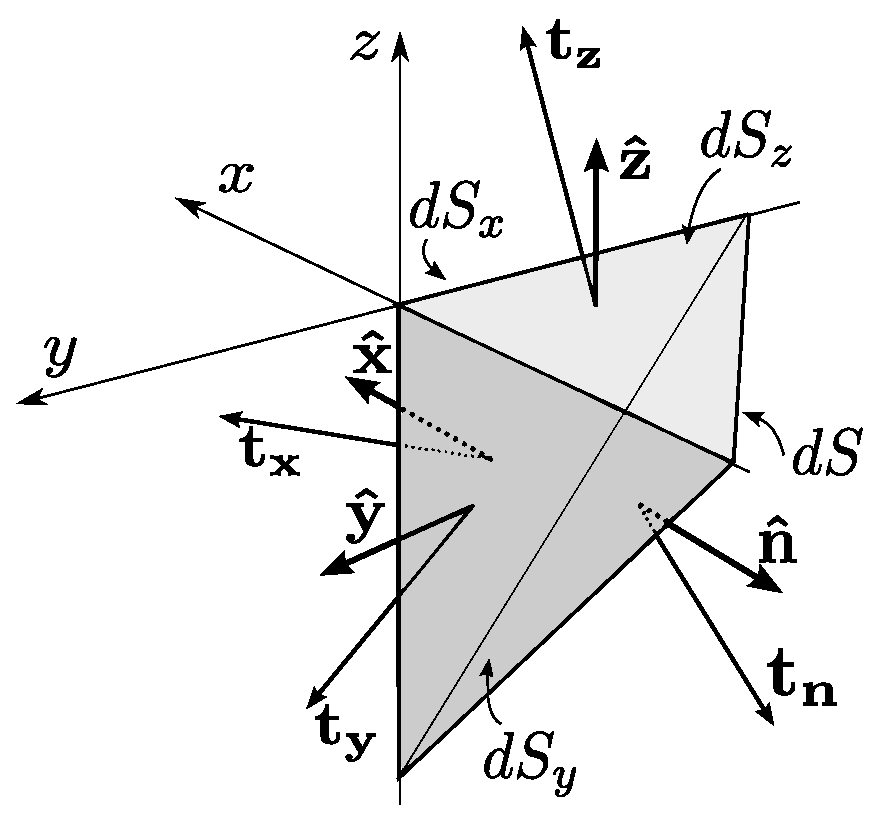
\includegraphics[width=0.60\textwidth]{./fig/cauchy.eps}
\caption{tetraedro di Cauchy}\label{fig:tetraedroCauchy}
\end{figure}

\begin{example}[Tensore di inerzia] Durante il corso di Meccanica Razionale si è visto che le componenti del tensore di inerzia espresse in un sistema di riferimento cartesiano ortogonale possono essere raccolte nella matrice simmetrica,
\begin{equation}
 \int_V \rho
 \begin{bmatrix}
   (y^2+z^2) &     -xy    &    -xz     \\ 
      -xy    &  (x^2+z^2) &    -yz     \\ 
      -xz    &     -yz    &  (x^2+y^2) \\ 
 \end{bmatrix}
\end{equation}
\begin{exercise}[Espressione tensoriale del tensore di inerzia] 
   Aiutandosi con un sistema di riferimento cartesiano, si dimostri che l'espressione tensoriale del tensore di inerzia è
    \begin{equation}
      \mathbb{I}_G = \int_V \rho \left[ |\bm{r}|^2 \mathbb{I} 
         - \bm{r} \otimes \bm{r} \right] \ ,
    \end{equation}
    essendo $\mathbb{I}$ il tensore identità del secondo ordine, $\bm{r}$ il raggio vettore tra un punto del corpo considerato e il punto $G$ rispetto al quale si sta calcolando il tensore di inerzia e l'integrale viene svolto su tutto il volume $V$ del corpo.
\end{exercise}
\end{example}

\begin{exercise}
    Dato il tensore simmetrico del secondo ordine definito nella base ortonormale $\{\bm{\hat{x}}, \bm{\hat{y}}\}$ dello spazio bidimensionale,
\begin{equation}
    \mathbb{A} = A_{xx} \bm{\hat{x}} \otimes \bm{\hat{x}} +
                 A_{xy} \bm{\hat{x}} \otimes \bm{\hat{y}} +
                 A_{xy} \bm{\hat{y}} \otimes \bm{\hat{x}} +
                 A_{yy} \bm{\hat{y}} \otimes \bm{\hat{y}} \ ,
\end{equation}
 si chiede di determinare la base ortonormale $\{\bm{\hat{\xi}},\bm{\hat{\eta}}\}$, che consente di esprimere il tensore $\mathbb{A}$ come 
\begin{equation}
    \mathbb{A} = A_{\xi \xi } \bm{\hat{\xi }} \otimes \bm{\hat{\xi }} +
                 A_{\eta\eta} \bm{\hat{\eta}} \otimes \bm{\hat{\eta}} \ , 
\end{equation}
cioé in forma diagonale.
\end{exercise}
%
\begin{figure}[h]
 \centering
 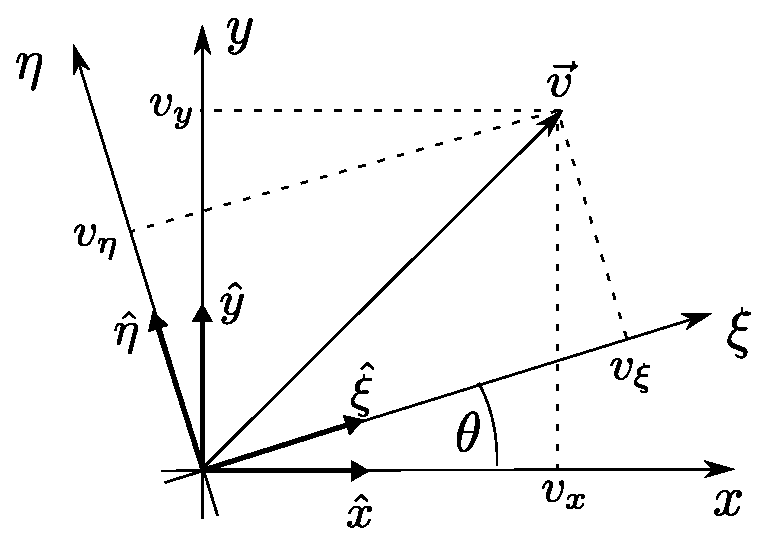
\includegraphics[width=0.5\textwidth]{./fig/rotation}
    \caption{Cambio di base: basi ortonormali.}\label{fig:tensor:rotation}
\end{figure}
Dati i due sistemi di riferimento raffigurati in figura \ref{fig:tensor:rotation}, la legge di trasformazione tra i vettori delle due basi è
\begin{equation}
 \begin{cases}
   \bm{\hat{\xi}} =  \cos{\theta} \bm{\hat{x}} + \sin{\theta} \bm{\hat{y}} \\
   \bm{\hat{\eta}} = -\sin{\theta} \bm{\hat{x}} + \cos{\theta} \bm{\hat{y}} \
 \end{cases} \qquad \rightarrow \qquad
    [ \bm{\hat{\xi}} | \bm{\hat{\eta}} ] = [ \bm{\hat{x}} | \bm{\hat{y}} ] \ T
\end{equation}
avendo indicato con $T$ la trasformazione lineare
\begin{equation}
 T = 
\begin{bmatrix}
 \cos{\theta} & \sin{\theta} \\
-\sin{\theta} & \cos{\theta} 
\end{bmatrix} \ ,
\end{equation}
e definendo $\tilde{T}=T^{-1}=T^T$, la sua inversa. Utilizzando la formula (\ref{eqn:t2t:t}), la trasformazione delle componenti di un tensore del secondo ordine diventa
\begin{equation}
    \tilde{A}_{ik} = \tilde{T}_{il} \tilde{T}_{km} A_{lm} \qquad , \qquad
    \tilde{A} = \tilde{T} A \tilde{T}^T \ ,
\end{equation}
non avendo fatto distinzione tra pedici e indici poiché si usano due basi ortonormali.
Si può quindi esplicitare l'ultima espressione per ricavare l'espressione delle componenti del tensore $\mathbb{A}$ nel nuovo sistema di riferimento,
 \begin{equation}
   \begin{bmatrix}
    A_{\xi \xi} & A_{\xi \eta} \\
    A_{\eta\xi} & A_{\eta\eta} \\
   \end{bmatrix} = 
   \begin{bmatrix} 
    \cos{\theta} & \sin{\theta} \\
   -\sin{\theta} & \cos{\theta} \\
   \end{bmatrix}
   \begin{bmatrix}
    A_{xx} & A_{xy} \\
    A_{yx} & A_{yy} \\
   \end{bmatrix}
   \begin{bmatrix} 
    \cos{\theta} &-\sin{\theta} \\
   \sin{\theta} & \cos{\theta} \\
   \end{bmatrix}
 \end{equation}
Svolgendo i conti e sfruttando la simmetria del tensore $\mathbb{A}$, $A_{xy} = A_{yx}$, si ottiene
  \begin{equation}
  \begin{aligned}
& \begin{bmatrix}
    A_{\xi \xi} & A_{\xi \eta} \\
    A_{\eta\xi} & A_{\eta\eta} \\
   \end{bmatrix} = \\ 
   & = \begin{bmatrix}
    A_{xx} \cos^2 \theta + A_{yy} \sin^2 \theta + 2 A_{xy} \cos \theta \sin \theta & 
      (-A_{xx} + A_{yy}) \cos \theta \sin \theta + A_{xy} ( \cos^2 \theta - \sin^2 \theta) \\
  (-A_{xx} + A_{yy}) \cos \theta \sin \theta + A_{xy} ( \cos^2 \theta - \sin^2 \theta) &
      A_{xx} \sin^2 \theta + A_{yy} \cos^2 \theta - 2 A_{xy} \cos \theta \sin \theta 
   \end{bmatrix} \ .
 \end{aligned}
 \end{equation}
Si osservi che la proprietà di simmetria del tensore è indipendente dalla base ortonormale utilizzata per esprimerne le componenti, $A_{\xi \eta} = A_{\eta \xi}$.
Per trovare l'angolo $\theta$ del quale bisogna ruotare il sistema di riferimento $\{\bm{\hat{\xi}},\bm{\hat{\eta}} \}$ affinché la componente $A_{\xi \eta}$ sia nulla, si impone
  \begin{equation}
   A_{\xi \eta} = 0 \ ,
  \end{equation}
ottenendo
  \begin{equation}
   0 = A_{xy} \cos {2\theta} - \dfrac{\sin{2\theta}}{2} (A_{xx}-A_{yy}) \quad \Rightarrow \quad
   \tan {2 \theta} = \dfrac{2 A_{xy}}{A_{xx}-A_{yy}} \ .
  \end{equation}
 %
 Il problema oggetto di questo esercizio è equivalente alla ricerca degli \textbf{assi principali di sforzo} per uno stato di sforzo piano, coincidenti con gli \textbf{autovettori} del tensore.\footnote{
     Gli autovettori di un tensore del secondo ordine $\mathbb{A}$ possono essere definiti come quei vettori $\bm{v}$ per i quali vale $\mathbb{A} \cdot \bm{v} = \lambda \bm{v}$ (autovettori ``destri'') oppure $\bm{v} \cdot \mathbb{A} = \lambda \bm{v}$ (autovettori ``sinistri''). Si ricorda che autovettori destri e sinistri coincidono nel caso in cui il tensore sia simmetrico. Infatti le due espressioni
\begin{equation}
\begin{aligned}
    \bm{v} \cdot \mathbb{A} & = v_i \bm{b}^i \cdot A^{jk} \bm{b}_j \otimes \bm{b}_k = 
    v_i A^{ik} \bm{b}_k \\
    \mathbb{A} \cdot \bm{v} & = A^{ij} \bm{b}_i \otimes \bm{b}_j \cdot v_k \bm{b}^k  = 
    A^{ij} v_j \bm{b}_i = A^{ki} v_i \bm{b}_k \ ,
\end{aligned}
\end{equation}
coincidono quando $A^{ij} = A^{ji}$. Nell'ultimo passaggio sono state modificate le lettere che identificano gli indici ripetuti per rendere più evidente il confronto tra le due espressioni.
Si ricorda inoltre che gli autovettori (opportunamente normalizzati) di un tensore simmetrico formano una base ortonormale $\{ \bm{v}^{(1)} , \dots , \bm{v}^{(N)} \}$, che può essere utilizzata per scrivere il tensore tramite la sua decomposizione spettrale
\begin{equation}
 \mathbb{A} = \lambda^{(1)} \bm{v}^{(1)} \otimes \bm{v}^{(1)} + \dots
              \lambda^{(N)} \bm{v}^{(N)} \otimes \bm{v}^{(N)} \ ,
\end{equation}
essendo $\lambda^{(i)}$ gli autovalori associati agli autovettori. Per convincersi della validità di tale decomposizione, è sufficiente moltiplicare con il ``prodotto punto'' il tensore $\mathbb{A}$ per uno dei vettori della base. Moltiplicandolo ad esempio per $\bm{v}^{(i)}$ e sfruttando l'ortogonalità dei vettori della base, si ottiene
\begin{equation}
\begin{aligned}
    \mathbb{A} \cdot \bm{v}^{(i)} & =
    \sum_{k=1}^{N} \left( \lambda^{(k)} \bm{v}^{(k)} \otimes \bm{v}^{(k)} \right) \cdot \bm{v}^{(i)}  = \\
& = \sum_{k=1}^{N} \left( \lambda^{(k)} \bm{v}^{(k)} \delta^{ik}\right) = 
    \lambda^{(i)} \bm{v}^{(i)} \ .
\end{aligned}
\end{equation}
 }
  Il risultato ricavato tramite le trasformazioni delle componenti dei tensori coincide con quello  già ottenuto nei corsi precedenti tramite l'equilibrio di un elementino di materiale, riassumibile nel diagramma del cerchio di Mohr. Avere in mente entrambi gli approcci può essere utile per non perdere il significato fisico di quello che si sta facendo.
%
\newline \noindent 
 La trasformazione delle componenti di un tensore in seguito al cambio di base può trovare molte altre applicazioni: un'altra applicazione ``da strutturista'' un po' più avanzato, consiste la determinazione delle caratteristiche meccaniche di elementi strutturali in materiale in composito, partendo dalle proprietà delle lamine che vengono usate per costruirlo.
 Ogni lamina ha caratteristiche meccaniche facilmente descrivibili nel proprio sistema di riferimento, la cui orientazione è determinata dalla direzione delle fibre, ad esempio, e che in generale è diversa da lamina a lamina. Le caratteristiche meccaniche del elemento strutturale vengono infine espresse in un suo sistema di riferimento globale, definito ad esempio dalla geometria del componente. 
%
\newline \noindent 
 Queste poche righe non hanno pretese di completezza, ma vogliono attirare l'interesse su quanto abbiamo visto nelle ultime ore, anche da parte di quelli che diventeranno ``strutturisti'' ma non solo.

\clearpage \newpage

\subsection{Cosa non è stato detto}
 Molte cose non sono state dette. Innanzitutto si è scelto di limitarsi alla rappresentazione di vettori e tensori utilizzando basi ortonormali dello spazio. Inoltre, è stato scelto di trattare i tensori su spazi forniti di prodotto interno e di non introdurre concetti di \textit{algebra esterna}, che permetterebbero di generalizzare l'operazione di prodotto vettoriale e l'operatore rotore incontrato nel calcolo vettoriale e ricavare il teorema di Stokes,
\begin{equation}
 \oint_{\partial \Omega} \omega = \int_\Omega d\omega ,
\end{equation}
 di cui viene solo riportata l'espressione matematica senza fornire alcun dettaglio. Il teorema del rotore e della divergenza sono casi particolari del teorema di Stokes, nel cui enunciato compaiono i concetti di forma differenziale $\omega$ e di derivata esterna $d \omega$.

 \noindent
Il materiale fornito rappresenta un compromesso tra il vuoto totale sul calcolo tensoriale (del quale l'affermazione ``un tensore è una matrice'' è la regina indiscussa) e un corso intero dedicato all'algebra e al calcolo tensoriale. Lo scopo dei cenni veloci ad argomenti non trattati qui è quello di ``mettere una pulce nell'orecchio'' di chi legge, di mettere a conoscenza il lettore dell'esistenza di alcuni argomenti che permettono di generalizzare le operazioni vettoriali presentate nei primi corsi di Algebra e di spiegare in maniera rigorosa alcuni comportamenti strani o inaspettati (come quelli che si possono osservare con il prodotto vettoriale e il rotore), senza scoperchiare dei vasi di Pandora che porterebbero questa introduzione lontana dal suo scopo.

\vspace{10pt}
 \noindent
 Per i più curiosi, viene messo a disposizione del materiale un più completo, che introduce concetti che non sono stati presentati qui e che generalizzano la trattazione, ma che la renderebbero inadatta ad essere svolta in poche ore per un pubblico formato da studenti del terzo anno di ingegneria, senza aggiungere particolari fondamentali per un utilizzo ``cosciente'' dei tensori durante questo corso e in quelli successivi.

 \subsubsection{Riferimenti.}  
 Il testo di Bowen e Wang, \textit{Introduction to vectors and tensors. Linear and multilinear algebra} può essere considerato un valido e completo riferimento, anche per il futuro. La lettura di questo testo non è sempre agevole e contiene sicuramente molto più di quanto sia indispensabile presentare in una prima e breve introduzione ai tensori, come è questa.
 Oltre alla sua qualità, è da apprezzare la disponibilità in rete dei due volumi, seguendo i seguenti collegamenti (sperando che siano ancora validi):
 
 \href{http://oaktrust.library.tamu.edu/bitstream/handle/1969.1/2502/IntroductionToVectorsAndTensorsVol1.pdf}
 {Vol. 1: Linear and Multilinear Algebra}
 
 \href{http://oaktrust.library.tamu.edu/bitstream/handle/1969.1/3609/IntroductionToVectorsAndTensorsVol2.pdf}
 {Vol. 2: Vector and Tensor Analysis}
 
% http://www.mat.unimi.it/users/carati/didattica/dispense/tensori.pdf
 
 
 \subsubsection{Cosa è utile ripassare.} Questa può essere una buona occasione per ripassare alcuni concetti di algebra lineare, tra i quali quello di spazio vettoriale (definizione e proprietà, dimensione e base, \dots), prodotto interno, linearità (e la differenza con l'essere ``affine''), alla luce di quanto visto in questi paragrafi introduttivi sui tensori e del fatto che le equazioni della fisica hanno carattere tensoriale.






% \section{Calcolo vettoriale e tensoriale in coordinate curvilinee}

Dopo aver introdotto alcuni concetti di algebra tensoriale nella sezione precedente, viene fatta una breve introduzione al calcolo tensoriale. In questa sezione vengono introdotte alcune definizioni e operatori differenziali necessari per descrivere campi (funzioni dipendenti dallo spazio) tensoriali. Si ricavano le espressioni in coordinate degli operatori rispetto a sistemi di coordinate curvilinee generali. Si introducono poi i sistemi di coordinate curvilinee ortogonali. Infine, si scrivono le espressioni di alcuni operatori differenziali e, come utile esempio per un corso di fluidodinamica, le equazioni di Navier-Stokes in un sistema di coordinate cilindriche.
Per aiutare la comprensione dell'argomento, i concetti generali verranno specializzati ad alcuni sistemi coordinate particolari, come le coordinate cartesiane o cilindriche.

Lavoriamo per semplicità in uno spazio tridimensionale, descritto completamente
 dalle tre coordinate $\left\{q^1, q^2, q^3\right\}$: il vettore posizione $\bm{x}$ sarà quindi una funzione
 delle tre coordinate $q^i$:
 \begin{equation}
  \bm{x} = \bm{x}(q^1, q^2, q^3)
 \end{equation}
 Si suppone che la trasformazione di coordinate da $\bm{x}$ a $\left\{q^1, q^2, q^3\right\}$ sia biunivoca. Vengono fornite ora le definizioni di curve coordinate, superfici coordinate e base naturale indotta dalla parametrizzazione dello spazio.

\begin{definition}[Curve coordinate]
 Le curve coordinate passanti per il punto $\bm{x}_0=\bm{x}(q_0^1, q_0^2, q_0^3)$ sono le curve ottenute al variare di una coordinata, tenendo fisse le altre due
 \begin{equation}
 \begin{cases}
  \ell_1 : \quad \bm{x} = \bm{x}(q^1, q_0^2, q_0^3) \\
  \ell_2 : \quad \bm{x} = \bm{x}(q_0^1, q^2, q_0^3) \\
  \ell_3 : \quad \bm{x} = \bm{x}(q_0^1, q_0^2, q^3) .
 \end{cases}
 \end{equation}
\end{definition}
 
\begin{definition}[Superfici coordinate]
 Le superfici coordinate passanti per il punto $\bm{x}_0=\bm{x}(q_0^1,q_0^2,q_0^3)$ sono le superficie descritte da due coordinate, tenendo fissa l'altra
 \begin{equation}
 \begin{cases}
  S_1 : \quad \bm{x} = \bm{x}(q_0^1, q^2, q^3) \\
  S_2 : \quad \bm{x} = \bm{x}(q^1, q_0^2, q^3) \\
  S_3 : \quad \bm{x} = \bm{x}(q^1, q^2, q_0^3) .
 \end{cases}
 \end{equation}
\end{definition}
 
\begin{definition}[Base naturale]
 Per ogni punto dello spazio tridimensionale $\bm{x}=\bm{x}(q^1,q^2,q^3)$, viene definita la base naturale $\{ \bm{b}_i \}_{i=1:3}$, i cui elementi sono le derivate parziali del vettore posizione rispetto alle coordinate $q^i$,
 \begin{equation}
  \bm{b}_i = \dfrac{\partial \bm{x}}{\partial q^i} . %\quad,\qquad \bm{b}^i = g^{ik} \bm{b}_k
 \end{equation}
\end{definition}
  La base reciproca $\{ \bm{b}^i \}_{i=1:3}$ della base naturale viene definita tramite la definizione (\ref{eqn:defBaseReciproca}), cioé $\bm{b}^i \cdot \bm{b}_j = \delta_j^i$.

\begin{example}[Coordinate cartesiane]
 La posizione di un punto nello spazio tridimensionale viene definito dalle tre componenti $(q^1, q^2, q^3)=(x,y,z)$ nel sistema di coordinate cartesiane. Le curve coordinate sono rette parallele agli assi, mentre le superfici coordinate sono dei piani perpendicolari agli assi. I vettori della base naturale sono i tre versori $\bm{\hat{b}}_x = {\hat{x}}$, $\bm{b}_y = \bm{\hat{y}}$, $\bm{b}_z = \bm{\hat{z}}$ allineati con le linee coordinate, costanti in tutto lo spazio.
\end{example}

\begin{example}[Coordinate cilindriche]
 La posizione di un punto nello spazio tridimensionale viene definito dalle tre componenti $(q^1, q^2, q^3)=(r,\theta,z)$ nel sistema di coordinate cilindriche, come raffigurato in figura \ref{fig:cylCoord}. Le curve coordinate $\bm{x}(r_0,\theta_0,z)$ sono delle linee parallele all'asse $z$, le curve coordinate $\bm{x}(r_0,\theta,z_0)$ sono delle circonferenze con centro sull'asse $z$, mentre le curve coordinate $\bm{x}(r,\theta_0,z_0)$ sono dei raggi (semirette) perpendicolari all'asse $z$. Le superfici coordinate $S_3=S_z$ sono dei piani perpendicolai all'asse $z$, le superfici coordinate $S_2=S_{\theta}$ sono dei cilindri con asse coincidente con l'asse $z$, le superfici coordinate $S_1 = S_r$ sono dei semipiani delimitati dall'asse $z$, come raffigurato in figura \ref{fig:cylCoord}\subref{fig:cylCoord:a}. I vettori della base naturale non sono costanti in spazio. \'E possibile calcolarli, esprimendo il vettore posizione in coordinate cartesiane e in coordinate cilindriche. In particolare $\bm{x} = x \bm{b}_x + y \bm{b}_y + z \bm{b}_z$, con
\begin{equation}
 \begin{cases}
  x = r \cos \theta \\   y = r \sin \theta \\ z = z .
 \end{cases}
\end{equation}
I vettori della base naturale possono essere calcolati inserendo queste espressioni nella formula che descrive la posizione nella base cartesiana, costante in spazio e quindi con derivate spaziali nulle. In figura \ref{fig:cylCoord}\subref{fig:cylCoord:b} sono rappresentati i vettori della base naturale
\begin{equation}
 \begin{cases}
  \bm{b}_1 = \bm{b}_r = \dfrac{\partial \bm{x}}{\partial r} = \cos \theta \bm{b}_x + \sin \theta \bm{b}_y  = \bm{\hat{r}} \\
  \bm{b}_2 = \bm{b}_{\theta} = \dfrac{\partial \bm{x}}{\partial \theta} = -r \sin \theta \bm{b}_x + r \cos \theta \bm{b}_y = r \bm{\hat{\theta}}\\
  \bm{b}_3 =  \bm{b}_z = \bm{\hat{z}} ,
 \end{cases}
\end{equation}
avendo introdotto i versori $\bm{\hat{r}} = \cos \theta \bm{b}_x + \sin \theta \bm{b}_y$, $\bm{\hat{\theta}}= -\sin \theta \bm{b}_x + \cos \theta \bm{b}_y$, comunemente utilizzati per descrivere i problemi in geometria cilindrica.
\begin{remark}
 I vettori della base naturale indotta dalle coordinate cilindriche \textbf{non} è costante nello spazio, è ortogonale (come vedremo nella prossima sezione) ma \textbf{non} è ortonormale e non ha dimensioni fisiche omogenee: mentre i vettori $\bm{b}_r$ e $\bm{b}_z$ hanno modulo 1, il vettore $\bm{b}_\theta$ ha modulo $r$ ed ha le dimensioni fisiche di una lunghezza.
\end{remark}
\end{example}

\begin{figure}
\subfloat[][\emph ]
   {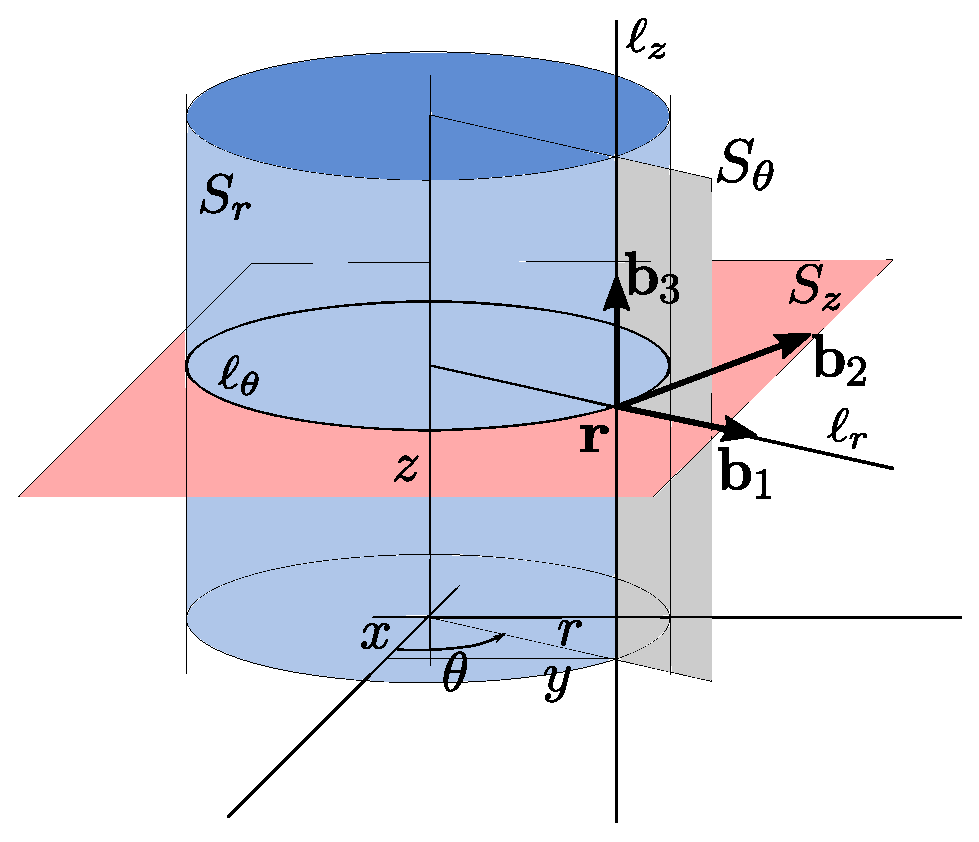
\includegraphics[width=0.45\textwidth]{./fig/cylindricalCoordinates.eps}\label{fig:cylCoord:a}}
\quad
\subfloat[][\emph ]
   {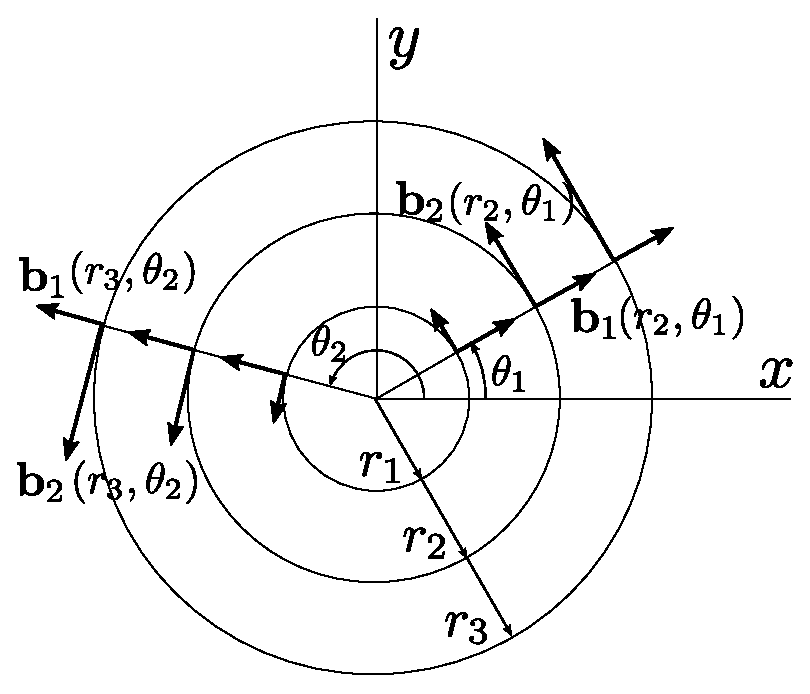
\includegraphics[width=0.45\textwidth]{./fig/cylindricalCoordinatesBasis.eps}\label{fig:cylCoord:b}}
\caption{Sistema di coordinate cilindriche.  \protect\subref{fig:cylCoord:a} Curve e superfici coordinate per un sistema di coordinate cilindriche. \protect\subref{fig:cylCoord:b} Rappresentazione bidimensionale della base naturale - coordinate polari.}\label{fig:cylCoord}
\end{figure}

%Ho appena definito \ref{fig:cylCoord},\ref{fig:cylCoord:a},\ref{fig:cylCoord:b}.

 \subsection{Tensore metrico.}
%
\vspace{15pt}
\begin{definition}[Tensore metrico]
 Il tensore metrico è un tensore del secondo ordine (o meglio un campo tensoriale, poiché in generale è funzione della coordinata spaziale) definito come il tensore le cui componenti covarianti $g_{ik}$ e contravarianti $g^{ik}$ sono rispettivamente i prodotti scalari dei vettori $\bm{b}_i$ della base naturale e dei vettori della base reciproca $\bm{b}^i$. Il tensore metrico $\bm{g}$ viene scritto nella base prodotto naturale e nella sua reciproca come
\begin{equation}
  \bm{g} = g_{ij} \bm{b}^i \otimes \bm{b}^j = g^{ij} \bm{b}_i \otimes \bm{b}_j ,
\end{equation}
con le componenti definite come
 \begin{equation}\label{eqn:defTensoreMetrico}
   g_{ij} = \bm{b}_i \cdot \bm{b}_j , \qquad g^{ij} = \bm{b}^i \cdot \bm{b}^j .
 \end{equation}
\end{definition}
%
% Si definisce il \textbf{tensore metrico} $\bm{g} = g_{ij} \bm{b}^i \otimes \bm{b}^j
% = g^{ij} \bm{b}_i \otimes \bm{b}_j $
% \begin{equation}
%   g_{ij} = \bm{b}_i \cdot \bm{b}_j \qquad , \qquad g^{ij} = \bm{b}^i \cdot \bm{b}^j
% \end{equation}
\begin{remark}
 Il tensore metrico è simmetrico.
\end{remark}
 Il tensore metrico caratterizza la geometria dello spazio (o meglio della varietà $\bm{x}(q^i)$ descritta dai parametri $q^i$). I concetti quali distanza, angolo, lunghezza di una curva possono essere espressi in funzione del tensore metrico $\bm{g}$. Ad esempio, è possibile scrivere la lunghezza $ds$ dell'elemento elementare $d\bm{x} = \dfrac{\partial \bm{x}}{\partial q^i} dq^i = \bm{b}_i dq^i$ come
 \begin{equation}
  ds^2 = |d\bm{x}|^2 = d\bm{x} \cdot d\bm{x} = \left( \bm{b}_i dq^i \right) \cdot \left(  \bm{b}_j dq^j\right) = \bm{b}_i \cdot \bm{b}_j dq^i dq^j = g_{ij} dq^i dq^j ,
 \end{equation}
 dove, come sempre, sono sottointese le sommatorie sugli indici ripetuti.
%
\noindent
Come già visto in precedenza, il tensore metrico risulta utile nel passaggio dalla componenti contravarianti a quelle 
 covarianti e viceversa, consentendo di esprimere un vettore della base $\{ \bm{b}_k \}$ nella base $\{ \bm{b}^k \}$ e viceversa tramite le (\ref{eqn:xxx})
 \begin{equation}
\bm{b}_i = g_{ik} \bm{b}^k , \quad \bm{b}^i = g^{ik} \bm{b}_k ,
 \end{equation}
 con $g_{ij} = \bm{b}_i \cdot \bm{b}_j$ e $g^{ij} = \bm{b}^i \cdot \bm{b}^j$. In maniera analoga è possibile passare dalle coordinate contravarianti a quelle covarianti e viceversa tramite le (\ref{eqn:xxx}). Ad esempio, per un vettore $\bm{v} = v^i \bm{b}_i = v_i \bm{b}^i$, 
 \begin{equation}
  v^i = g^{ik} v_k , \qquad v_i = g_{ik} v^k .
 \end{equation}
 Sempre secondo le (\ref{eqn:xxx}), per un tensore del secondo ordine $\bm{S}= S^{ij} \bm{b}_i \otimes \bm{b}_j = 
    S^{i\ }_{\ j} \bm{b}_i \otimes \bm{b}^j =
    S^{\ j}_{i\ } \bm{b}^i \otimes \bm{b}_j = 
    S_{ij} \bm{b}^i \otimes \bm{b}^j$ si ottiene
 \begin{equation}
  S^{ij} = g^{jk} S^{i\ }_{\ k} = g^{ik} S^{\ \ j}_{k\ } = g^{ik} g^{jl} S_{kl} .
 \end{equation}
%
\begin{example}[Coordinate cartesiane]
    Poichè i vettori della base naturale sono costanti e ortonormali in tutto lo spazio, dalla definizione (\ref{eqn:defTensoreMetrico}) segue che il tensore metrico $g_{ik}$ è uguale all'identità.
 La lunghezza dell'elemento di linea infinitesimo è uguale a
\begin{equation}
    ds^2 = |d\bm{x}|^2 = dx^2 + dy^2 + dz^2 \ .
\end{equation}
\end{example}
%
\begin{example}[Coordinate cilindriche]
 Svolgendo i prodotti scalari tra i vettori della base del sistema di coordinate cilindriche, le componenti $g_{ik}$ del tensore metrico possono essere raccolte nella matrice.
\begin{equation}
 \begin{bmatrix} g_{rr} & g_{r\theta} & g_{rz} \\
 g_{\theta r} & g_{\theta \theta} & g_{\theta z} \\
 g_{z r} & g_{z \theta} & g_{zz} \\ \end{bmatrix} = 
 \begin{bmatrix} 1 & 0 & 0 \\ 0 & r^2 & 0 \\ 0 & 0 & 1  \\ \end{bmatrix} .
\end{equation}
 Il tensore metrico è diagonale, poichè la base è ortogonale. Le componenti covarianti $g^{ik}$ del tensore metrico si ottengono dall'inversione dei simboli $g_{ik}$
\begin{equation}
 \begin{bmatrix} g^{rr} & g^{r\theta} & g^{rz} \\
 g^{\theta r} & g^{\theta \theta} & g^{\theta z} \\
 g^{z r} & g^{z \theta} & g^{zz} \\ \end{bmatrix} = 
 \begin{bmatrix} 1 & 0 & 0 \\ 0 & r^{-2} & 0 \\ 0 & 0 & 1  \\ \end{bmatrix} .
\end{equation}
La base reciproca è $\bm{b}^r = \bm{b}_r$, $\bm{b}^{\theta} = r^{-2} \bm{b}_{\theta} = r^{-1} \bm{\hat{\theta}}$, $\bm{b}^z = \bm{b}_z$.
 La lunghezza dell'elemento di linea infinitesimo è uguale a
\begin{equation}
    ds^2 = |d\bm{x}|^2 = dr^2 + r^2 d\theta^2 + dz^2 \ .
\end{equation}
\end{example}


% \paragraph{Componenti contravarianti, covarianti e fisiche.} \dots
 
 \subsection{Simboli di Christoffel.} 
I vettori della base naturale $\bm{b}_i$ sono definiti come le derivate parziali del vettore posizione $\bm{x}$ rispetto alle coordinate $q^i$ utilizzate per descrivere lo spazio. In generale, quindi anche i vettori della base naturale non sono costanti nello spazio, ma sono funzioni delle coordinate $q^i$. Se i vettori della base variano dello spazio, le loro derivate rispetto ai parametri $q^i$ non sono nulle e possono essere espresse nella base naturale e nella base reciproca come
\begin{equation}\label{eqn:dbdq}
 \dfrac{\partial \bm{b}_i}{\partial q^j} = \Gamma_{ij}^k \bm{b}_k ,
\end{equation}
 dove stati introdotti i simboli di Christoffel di secondo tipo $\Gamma^{k}_{ij}$. In particolare, dalla (\ref{eqn:dbdq}), i simboli di Christoffel di secondo tipo $\Gamma^{k}_{ij}$ possono essere definiti come la $k$-esima componente contravariante della derivata $\partial \bm{b}_i/\partial q^j$. Sfruttando la definizione di base reciproca, è possibile calcolare i simboli di Christoffel dalle (\ref{eqn:dbdq}) come
\begin{equation}
  \Gamma^{k}_{ij} = \dfrac{\partial \bm{b}_i}{\partial q^j} \cdot \bm{b}^k .
\end{equation}
Essendo le componenti delle derivate prime dei vettori della base naturale, a sua volta derivate prime del vettore posizione, i simboli di Christoffel rappresentano le componenti delle derivate seconde del vettore posizione $\bm{x}$ rispetto alle coordinate $q^i$,
\begin{equation}
 \Gamma_{ji}^k \bm{b}_k = 
 \dfrac{\partial \bm{b}_j}{\partial q^i} =\dfrac{\partial^2 \bm{x}}{\partial q^j \partial q^i} =
 \dfrac{\partial^2 \bm{x}}{\partial q^i \partial q^j} = \dfrac{\partial \bm{b}_i}{\partial q^j}= \Gamma_{ij}^k \bm{b}_k ,
\end{equation}
dove l'uguaglianza delle derivate seconde miste è verificata sotto le ipotesi del \textit{teorema di Schwarz}. Uguagliando le componenti alle estremità dell'uguaglianza precedente, si ottengono le condizioni di simmetria per i simboli di Christoffel,
\begin{equation}
 \Gamma_{ji}^k = \Gamma_{ij}^k \ .
\end{equation}
\begin{remark}
 I simboli di Christoffel \textbf{non} costituiscono le componenti di un tensore, poichè non seguono la (\ref{eqn:t2t:t}) nel cambio di sistemi di coordinate.
\end{remark}

\begin{example}[Coordinate cartesiane]
 Poichè i vettori della base naturale sono costanti in tutto lo spazio, i simboli di Christoffel per il sistema di coordinate cartesiane sono identicamente nulli.
\end{example}
\begin{example}[Coordinate cilindriche]
 Vengono calcolati i simboli di Christoffel di secondo tipo, che verranno poi utilizzati in seguito). Da un calcolo diretto dei simboli di Christoffel di secondo tipo, si ottiene che gli unici simboli di Christoffel diversi da zero sono
\begin{equation}
 \Gamma^2_{21} = \Gamma^2_{12} = r^{-1} , \quad \Gamma^1_{22} = - r ,
\end{equation}
dove l'indice 1 è associato alla coordinata $r$, l'indice 2 alla coordinata $\theta$. Infatti
\begin{equation}
\begin{aligned}
 \Gamma_{21}^2 = \Gamma_{12}^2  & = \dfrac{\partial \bm{b}_1}{\partial q^2} \cdot \bm{b}^2 = \dfrac{\partial \bm{\hat{r}}}{\partial \theta} \cdot( r^{-1} \bm{\hat{\theta}} ) = \bm{\hat{\theta}} \cdot (r^{-1} \bm{\hat{\theta}}) = r^{-1} \\
 \Gamma_{22}^1  & = \dfrac{\partial \bm{b}_2}{\partial q^2} \cdot \bm{b}^1 = \dfrac{\partial (r \bm{\hat{\theta}})}{\partial \theta} \cdot \bm{\hat{r}} = - r \bm{\hat{r}} \cdot \bm{\hat{r}} = - r . \\
\end{aligned}
\end{equation}
\end{example}

% +++++++++++++++++++++++++++++++++++++++++++++++++++++++++++++++++++++++++++++++++
\section{Operatori differenziali}\label{ch:operatoriDiff}
 % \paragraph{Derivata covariante}
 % \paragraph{Operatori differenziali}
 % \paragraph{Gradiente}
 % \paragraph{Divergenza}
 % \paragraph{Laplaciano}
 % \paragraph{Rotore}
 % \paragraph{Operatore di advezione}
In questo paragrafo vengono definiti alcuni operatori differenziali sui campi tensoriali, cioè tensori che sono funzioni dello spazio. Un operatore è una funzione che prende come argomento l'oggetto al quale viene applicato, per restituirne un altro. In termini generali, un operatore $P: U \rightarrow V$, prende un elemento di $U$ e ne restituisce uno di $V$,
\begin{equation}\label{def:operatore}
  \bm{v} = P(\bm{u}),
\end{equation}
con $\bm{u} \in U$, $\bm{v} \in V$. Per ottenere un vettore di $\bm{v} \in V$, l'operatore $P$ deve avere come argomento (deve essere applicato a) un elemento $\bm{u} \in U$. Se $P$ è un operatore lineare spesso si possono omettere le parentesi e indicare semplicemente $\bm{v}=P\bm{u}$.
L'ordine di un operatore coincide con il massimo ordine delle derivate (in questo caso spaziali) contenute nella definizione dell'operatore. Inizialmente vengono introdotti gli operatori di primo ordine che non richiedono l'introduzione di prodotti esterni (parenti dei prodotti vettoriali): gradiente, divergenza e operatore di advezione. Viene poi introdotto l'operatore di rotore di un campo vettoriale, limitandosi a sistemi di coordinate cartesiane. Infine viene introdotto il laplaciano, un operatore del secondo ordine definito come la divergenza del gradiente.
\begin{remark}
 Diversi autori usano convenzioni diverse per la definizione degli operatori differenziali, come ad esempio la divergenza di un tensore di secondo ordine. Nel caso di tensori simmetrici (come sono i tensori degli sforzi per materiali non polari), le due diverse definizioni di divergenza di un tensore portano allo stesso risultato, grazie alla simmetria del tensore. 
\end{remark}

\subsection{Gradiente}
L'operatore di gradiente è connesso alla derivata direzionale di un campo tensoriale.
L'operatore di gradiente alza di 1 l'ordine del tensore al quale viene applicato.
\begin{operator}[Gradiente] 
    In particolare, nel punto $\bm{x}$ la derivata direzionale di un tensore $\bm{T}$ in una qualsiasi direzione $\bm{c}$ di un campo tensoriale è il prodotto scalare tra il gradiente del tensore e il vettore $\bm{c}$,
 \begin{equation}\label{eqn:grad:def}
   \bm{c} \cdot \bm{\nabla} \bm{T}(\bm{x}) = \left. \dfrac{d}{d\alpha} \bm{T}(\bm{x}+\alpha\bm{c})\right|_{\alpha=0} \ .
 \end{equation}
\end{operator}
%
\noindent
Il gradiente del tensore $\bm{T}$ può essere scritto sfruttando la definizione della base naturale e della sua reciproca come
%\begin{fBox}
 \begin{equation}\label{eqn:grad:natural}
  \bm{\nabla} \bm{T} = \bm{b}^i \otimes \dfrac{\partial \bm{T}}{\partial q^i} ,
 \end{equation}
%\end{fBox}
dove i vettori $\bm{b}^i$ sono quelli della base reciproca della base naturale e, come al solito, è sottintesa la sommatoria sugli indici ripetuti.
%  \'E possibile indicare l'operatore gradiente con $G$, senza applicarlo ad alcun tensore, rimuovendo l'argomento dalla (\ref{eqn:grad:natural}),
%  \begin{equation}\label{eqn:grad:natural:operator}
%   G \underline{\hspace{8pt}} = \text{grad} \ \underline{\hspace{8pt}} = \dfrac{\partial \underline{\hspace{8pt}}}{\partial q^i} \otimes \bm{b}^i ,
%  \end{equation}
%  avendo lasciato lo spazio $\underline{\hspace{8pt}}$ per inserire l'argomento dell'operatore gradiente e avendo omesso le parentesi poichè il gradiente è un operatore lineare. Il gradiente di un campo tensoriale $\bm{T}$ viene ottenuto semplicemente inserendo $\bm{T}$ negli spazi indicati nella (\ref{eqn:grad:natural:operator}).
%
 \noindent
 Il gradiente di un tensore di ordine $r$ ha ordine $r+1$. Per esempio, il gradiente di un campo scalare $f$ è il vettore $\bm{\nabla} f$
 \begin{equation}\label{eqn:grad:scalar}
  \bm{\nabla} f = \bm{b}^i \dfrac{\partial f}{\partial q^i} = \dfrac{\partial f}{\partial q^i} \bm{b}^i = \dfrac{\partial f}{\partial q^k} g^{ik} \bm{b}_i \ ,
 \end{equation}
 avendo utilizzato la relazione $\bm{b}^i = g^{ik} \bm{b}_k$ tra i vettori di una base e quelli della sua reciproca (e avendo ``invertito'' gli indici ripetuti, che vengono saturati dalle sommatorie).
 Il gradiente di un campo vettoriale è il campo tensoriale del secondo ordine che viene scritto nella base naturale come
 \begin{equation}\label{eqn:grad:vector}
   \bm{\nabla} \bm{v} = \bm{b}^i \otimes \dfrac{\partial \bm{v}}{\partial q^i} = \left[ \dfrac{\partial v^i}{\partial q^k} + \Gamma_{lk}^i v^l \right] \bm{b}^k \otimes \bm{b}_i ,
 \end{equation}
dove sono sottointese le sommatorie sugli indici ripetuti.
\begin{exercise}[Gradiente di un campo vettoriale] Ricavare l'espressione (\ref{eqn:grad:vector}) del gradiente di un campo scalare.

 \vspace{5pt}\noindent
 \textbf{Soluzione.} \'E possibile ricavare questa espressione tramite calcolo diretto delle derivate parziali di $\bm{v}$, ricordandosi la definizione dei simboli di Christoffel e, alla fine, ricordandosi che è possibile scambiare gli indici che vengono saturati da sommatoria, \vspace{-5pt}
\begin{equation}
\begin{aligned}
    \bm{\nabla} \bm{v} & = \bm{b}^k \otimes \dfrac{\partial \bm{v}}{\partial q^k} % = \\
       = \bm{b}^k \otimes \dfrac{\partial (v^i \bm{b}_i)}{\partial q^k}  = \\
     & = \bm{b}^k \otimes \left[ \dfrac{\partial v^i }{\partial q^k} \bm{b}_i +
       v^i \dfrac{\partial \bm{b}_i}{\partial q^k} \right] % = \\
       = \bm{b}^k \otimes \left[ \dfrac{\partial v^i }{\partial q^k} \bm{b}_i +
       v^i \Gamma^{l}_{ik} \bm{b}_l \right] = \\
     & = \left[ \dfrac{\partial v^i }{\partial q^k} +
       v^l \Gamma^{i}_{lk} \right] \bm{b}^k \otimes \bm{b}_i = \nabla_k v^i \bm{b}^k \otimes \bm{b}_i \ ,
\end{aligned}
\end{equation}
dove è stata introdotta la derivata covariante $\nabla_k v^i$ della componente $v^i$ del vettore, rispetto alla coordinata $q^k$.
\end{exercise}

\noindent
Il gradiente di un campo tensoriale del secondo ordine $\bm{S}$ è il campo tensoriale del terzo ordine
 \begin{equation}\label{eqn:grad:tensor2}
   \bm{\nabla} \bm{S} = \left[ \dfrac{\partial S^{ij}}{\partial q^k} + \Gamma_{kl}^i S^{lj} + \Gamma_{kl}^j S^{il} \right]
                \bm{b}^k \otimes \bm{b}_i \otimes \bm{b}_j =: \nabla_k S^{ij} \bm{b}^k \otimes \bm{b}_i \otimes \bm{b}_j \ ,
 \end{equation}
 dove è stata introdotta la definizione di \textbf{derivata covariante} $\nabla_k S^{ij}$ della componente $S^{ij}$ rispetto alla coordinata $q^k$, come generalizzazione delle derivate parziali. Un campo tensoriale è costante nello spazio se sono nulle tutte le sue derivate covarianti.
\begin{exercise}[Gradiente di un campo tensoriale del secondo ordine]
 Aiutandosi con la dimostrazione data per il gradiente di un campo vettoriale, dimostrare che il gradiente di un campo tensoriale del secondo ordine ha l'espressione (\ref{eqn:grad:tensor2}) utilizzando la base naturale e la sua reciproca.
\end{exercise}
%
\begin{example}[Coordinate cartesiane]
 Poichè la base naturale e la sua reciproca coincidono con la base ortonormale $\{\bm{\hat{x}}, \bm{\hat{y}}, \bm{\hat{z}}\}$ e tutti i simboli di Christoffel per le coordinate cartesiane sono nulli, dalla (\ref{eqn:grad:scalar}) si ottiene la forma già nota del gradiente di un campo scalare $f$
\begin{equation}
 \bm{\nabla} f = \dfrac{\partial f}{\partial x} \bm{\hat{x}} +
                 \dfrac{\partial f}{\partial y} \bm{\hat{y}} +
                 \dfrac{\partial f}{\partial z} \bm{\hat{z}} .
\end{equation}
Il gradiente di un vettore $\bm{v} = v^1 \bm{b}_1 +v^2 \bm{b}_2 + v^3 \bm{b}_3  = v_x \bm{\hat{x}} + v_y \bm{\hat{y}} + v_z \bm{\hat{z}}$ è
\begin{equation}
 \begin{aligned}
  \bm{\nabla} \bm{v} = & \p{v_x}{x} \bh{x}\ot\bh{x} + 
                         \p{v_y}{x} \bh{x}\ot\bh{y} +
                         \p{v_z}{x} \bh{x}\ot\bh{z} + \\ 
                     + & \p{v_x}{y} \bh{y}\ot\bh{x} + 
                         \p{v_y}{y} \bh{y}\ot\bh{y} +
                         \p{v_z}{y} \bh{y}\ot\bh{z} + \\ 
                     + & \p{v_x}{z} \bh{z}\ot\bh{x} + 
                         \p{v_y}{z} \bh{z}\ot\bh{y} +
                         \p{v_z}{z} \bh{z}\ot\bh{z} , \\ 
 \end{aligned}
\end{equation}
 le cui componenti possono essere raccolte nella matrice
\begin{equation}
 \begin{bmatrix}
  \p{v_x}{x}  & 
  \p{v_y}{x}  &
  \p{v_z}{x}   \\ 
  \p{v_x}{y}  & 
  \p{v_y}{y}  &
  \p{v_z}{y}   \\ 
  \p{v_x}{z}  & 
  \p{v_y}{z}  &
  \p{v_z}{z}   \\ 
 \end{bmatrix} \ ,
\end{equation}
avendo associato l'indice di riga al primo vettore della base prodotto e l'indice di colonna al secondo vettore della base prodotto.
\end{example}
%
\begin{example}[Coordinate cilindriche]
 Il gradiente in coordinate cilindriche di un campo scalare $f$ può essere scritto nella base ortonormale $\{ \bh{r}, \bh{\theta},\bh{z} \}$ come
\begin{equation}
 \bm{\nabla} f = \p{f}{r} \bh{r} + \dfrac{1}{r}\p{f}{\theta} \bh{\theta} +
   \p{f}{z} \bh{z} ,
\end{equation}
 avendo utilizzato la (\ref{eqn:grad:scalar}) ed essendosi ricordati che $\bh{b}_2 = \bh{\theta} / r$. Da quest'ultima relazione tra i vettori delle basi naturale e ortonormale si ottiene il legame $v^2 = r v_{\theta}$ tra le componenti del vettore $\bm{v} = v^1 \bh{b}_1 + v^2 \bh{b}_2 + v^3 \bh{b}_3 = v_r \bh{r} + v_{\theta} \bh{\theta} + v_z \bh{z}$ espresse in queste basi. Utilizzando queste relazioni nella formula (\ref{eqn:grad:vector}) del gradiente di un campo vettoriale, è possibile scrivere
\begin{equation}
\begin{aligned}
    \bm{\nabla} \bm{v} & = \left[ \dfrac{\partial v^i}{\partial q^k} + \Gamma_{lk}^i v^l \right] \bm{b}^k \otimes \bm{b}_i = \\
     & = \frac{\partial v^1}{\partial q^1}                                   \bm{b}^1 \otimes \bm{b}_1   + 
        \left( \frac{\partial v^1}{\partial q^2} + \Gamma_{22}^1 v^2 \right) \bm{b}^2 \otimes \bm{b}_1   + 
        \frac{\partial v^1}{\partial q^3}                                    \bm{b}^3 \otimes \bm{b}_1   + \\
     & + \left( \frac{\partial v^2}{\partial q^1} + \Gamma_{21}^2 v^2 \right)\bm{b}^1 \otimes \bm{b}_2   + 
        \left( \frac{\partial v^2}{\partial q^2} + \Gamma_{12}^2 v^1 \right) \bm{b}^2 \otimes \bm{b}_2   + 
        \frac{\partial v^2}{\partial q^3}                                    \bm{b}^3 \otimes \bm{b}_2   + \\
     & + \frac{\partial v^3}{\partial q^1}                                   \bm{b}^1 \otimes \bm{b}_3   + 
        \frac{\partial v^3}{\partial q^2}                                    \bm{b}^2 \otimes \bm{b}_3   + 
        \frac{\partial v^3}{\partial q^3}                                    \bm{b}^3 \otimes \bm{b}_3   = \\
     & = \frac{\partial v_r}{\partial r}                                           \bm{\hat{r}}      \otimes \bm{\hat{r}}       + 
        \frac{1}{r}\left( \frac{\partial v_r}{\partial \theta} - v_\theta \right)  \bm{\hat{\theta}} \otimes \bm{\hat{r}}       + 
        \frac{\partial v_r}{\partial z}                                            \bm{\hat{z}}      \otimes \bm{\hat{r}}       + \\
     & +  \frac{\partial v_\theta}{\partial r}                                     \bm{\hat{r}}      \otimes \bm{\hat{\theta}}  + 
        \frac{1}{r}\left( \frac{\partial v_\theta}{\partial \theta} +  v_r \right) \bm{\hat{\theta}} \otimes \bm{\hat{\theta}}  + 
        \frac{\partial v_\theta}{\partial z}                                       \bm{\hat{z}}      \otimes \bm{\hat{\theta}}  + \\
     & + \frac{\partial v_z}{\partial r}                                           \bm{\hat{r}}      \otimes \bm{\hat{z}}       + 
        \frac{1}{r}\frac{\partial v_z}{\partial \theta}                            \bm{\hat{\theta}} \otimes \bm{\hat{z}}       + 
        \frac{\partial v_z}{\partial z}                                            \bm{\hat{z}}      \otimes \bm{\hat{z}}        ,
\end{aligned}
\end{equation}
 avendo utilizzato i valori dei simboli di Christoffel ricavati in precedenza. Si noti come l'annullarsi delle derivate parziali delle componeti del vettore non implichi l'uniformità (costanza in spazio e quindi gradiente nullo) del campo vettoriale: devono annullarsi le derivate covarianti poichè un campo vettoriale uniforme espresso in coordinate cilindriche (come in ogni altro sistema di coordinate diverso da quello cartesiano) non ha componenti costanti in spazio.
\end{example}

% ===============================================================
\subsection{Divergenza}
L'operatore divergenza è associato all'idea di densità di flusso\footnote{Si può ricavare questa interpretazione dal teorema della divergenza.} e può essere definito come contrazione del gradiente del campo al quale viene applicata. L'operatore di divergenza quindi abbassa di 1 (il gradiente alza di 1 l'ordine, la contrazione di due indici lo abbassa di 2) l'ordine del campo tensoriale al quale è applicata. Non può quindi essere applicata a un campo scalare (tensore di ordine 0).
\begin{operator}[Divergenza]
 La divergenza di un campo tensoriale è definito dalla contrazione degli ultimi due indici del gradiente del campo tensoriale stesso.
\begin{equation}\label{eqn:div:def}
 \bm{\nabla} \cdot \bm{T} = \bm{C}^{1}_{2} \big( \bm{\nabla} \bm{T} \big)\  .
\end{equation}
\end{operator}
% L'operatore di divergenza abbassa di 1 l'ordine del tensore al quale viene applicato: la divergenza di un tesnore di ordine $r$ ha ordine $r-1$. Non può quindi essere applicato a un campo scalare (tensore di ordine 0).
La divergenza di un campo vettoriale espresso nella base naturale è
\begin{equation}\label{eqn:div:vector}
 \bm{\nabla} \cdot\bm{v} = \dfrac{\partial v^{i}}{\partial q^i} + \Gamma_{il}^i v^{l} = \nabla_i v^{i} .
\end{equation}
 La divergenza di un tensore $\bm{S}$ del secondo ordine è il campo vettoriale $\bm{\nabla} \cdot \bm{S}$ che viene scritto nella base naturale come
 \begin{equation}\label{eqn:div:tensor2}
  \bm{\nabla} \cdot \bm{S} = \left[ \dfrac{\partial S^{ij}}{\partial q^i} + \Gamma_{il}^i S^{lj} + \Gamma_{il}^j S^{il} \right] \bm{b}_j .
 \end{equation}
%
Questo operatore può essere espresso tramite la derivata covariante come
\begin{equation}
 \bm{\nabla} \cdot \bm{S} = \nabla_i S^{ij} \bm{b}^j ,
\end{equation}
e può essere pensato come il prodotto ``dot'' tra il ``vettore formale'' $\bm{\nabla} = \nabla_k \bm{b}^k$ e il tensore $S^{ij} \bm{b}_i \otimes \bm{b}_j$,
\begin{equation}
      \bm{\nabla} \cdot \bm{S} = (\nabla_k \bm{b}^k) \cdot ( S^{ij} \bm{b}_i \otimes \bm{b}_j ) = \nabla_k S^{ij} \underbrace{\bm{b}^k \cdot \bm{b}_i}_{\delta^k_i} \otimes \bm{b}_j  = 
     \nabla_i S^{ij} \bm{b}_j \ . 
\end{equation}
%

\begin{exercise}
 Utilizzando la definizione di divergenza e l'espressione (\ref{eqn:grad:vector}) del gradiente di un campo vettoriale, ricavare l'espressione (\ref{eqn:div:vector}) di un campo vettoriale.
\end{exercise}
\begin{exercise}
 Utilizzando la definizione di divergenza e l'espressione (\ref{eqn:grad:tensor2}) del gradiente di un campo vettoriale, ricavare l'espressione (\ref{eqn:div:tensor2}) di un campo vettoriale.
\end{exercise}

% \noindent
% La divergenza di un vettore $\bm{v}$, questa definizione si riduce alla traccia\footnote{La traccia di un tensore è un \textit{invariante}, cioè non varia cambiando la base dello spazio, definito come la somma degli elementi della diagonale}
% del gradiente
% \begin{equation}
%  \text{div} \bm{v} = \bm{\nabla} \cdot \bm{v}  = \text{tr}(\bm{\nabla}\bm{v})
% \end{equation}
\begin{example}[Coordinate cartesiane]
 Poichè i simboli di Christoffel sono identicamente nulli e i vettori della base naturale coincidono con la terna ortonormale $\{ \bh{x}, \bh{y}, \bh{z}\}$ nei sistemi di coordinate cartesiane, dalla (\ref{eqn:div:vector}) si ottiene la forma già nota della divergenza di un campo vettoriale $\bm{v}$ 
\begin{equation}
 \bm{\nabla} \cdot \bm{v} = \p{v_x}{x} + \p{v_y}{y} + \p{v_z}{z}.
\end{equation}
\end{example}
\begin{example}[Coordinate cilindriche]
In coordinate cilindriche gli unici simboli di Christoffel non nulli sono $\Gamma^2_{12} = \Gamma^2_{21} = r^{-1}$, $\Gamma^1_{22} = -r$. Utilizzando la (\ref{eqn:div:vector}), la divergenza di un campo vettoriale $\bm{v} = v^1 \bh{b}_1 + v^2 \bh{b}_2 + v^3 \bh{b}_3 = v_r \bh{r} + v_{\theta} \bh{\theta} + v_z \bh{z}$ viene scritta in coordinate cilindriche come
\begin{equation}
\begin{aligned}
 \text{div} \bm{v} = \bm{\nabla} \cdot \bm{v} & =
  \p{v^1}{q^1} + \p{v^2}{q^2} + \Gamma_{12}^2 v^1 + \p{v^3}{q^3} = \\
  & = \p{v_r}{r} + \p{ (v_{\theta}/r) }{\theta} + \dfrac{v_r}{r} + \p{v_z}{z} = \\	
  & = \dfrac{1}{r}\p{( r v_r)}{r} + \dfrac{1}{r}\p{v_{\theta}}{\theta} + \p{v_z}{z}.
\end{aligned}
\end{equation}
\end{example}

\begin{remark}
Utilizzando il lemma \ref{lemma:stokes:2} e l'espressione del vettore sforzo (\ref{eqn:tensor:stressTensor}) in componenti cartesiane (per le quali la base reciproca coincide con la base ortonormale naturale e le componenti contravarianti e covarianti coincidono con le variabili fisiche, vedere \S\ref{ch:tensori:coordinate_ortogonali}), è possibile trasformare il contributo degli sforzi di superficie $\bm{t_n}$ in un integrale di volume,
\begin{equation}
  \oint_S \bm{t_n} = \oint_S \bh{n} \cdot \bm{T} = \oint_S n_i T_{ij} = \int_V \partial_i T_{ij} = \int_V \bm{\nabla} \cdot \bm{T} ,
\end{equation}
 avendo indicato la superficie chiusa del volume $V$ con $S=\partial V$ e riconosciuto l'espressione in componenti cartesiane (per le quali le derivate covarianti coincidono con le derivate parziali) dell'operatore $\bm{\nabla} \cdot$ applicato al tensore degli sforzi $\bm{T}$. Poiché il tensore degli sforzi per continui non polari è simmetrico, la confusione generata dalle due definizioni diverse di divergenza usate da alcuni autori è solo apparente quando applicata al tensore degli sforzi.
\end{remark}

\noindent
\begin{remark}
    Le equazioni vettoriali (o tensoriali) e le identità vettoriali (o tensoriali) possono essere scritte nel sistema di riferimento più conveniente. Durante il corso di Fluidodinamica si incontreranno alcune \textbf{identità vettoriali} utili all'elaborazione delle equazioni. Per chi volesse provare a dimostrarle, o dimostrarne almeno qualcuna, può usare le coordinate cartesiane, per le quali i simboli di Christoffel sono nulli e le derivate covarianti si riducono alle derivate parziali. \textbf{La validità di un'identità vettoriale non dipende dal sistema di riferimento in cui viene scritta}. Per fornire un primo esempio, si dimostra che
 \begin{equation}
  \bm{\nabla} \cdot (a \bm{v}) = \bm{\nabla} a \cdot \bm{v} + a \bm{\nabla} \cdot \bm{v} ,
 \end{equation}
 dove $a$ e $\bm{v}$ sono rispettivamente un campo scalare e vettoriale definiti nello spazio $\mathbb{R}^2$. Il campo vettoriale viene scritto in coordinate cartesiane come $\bm{v} = v_x \bh{x} + v_y \bh{y}$. Da un calcolo diretto, si ottiene
 \begin{equation}
 \begin{aligned}
   \bm{\nabla} \cdot (a \bm{v}) & = \p{(a v_x)}{x} + \p{(a v_y)}{y} = \\
    & = \p{a}{x} v_x + a \p{v_x}{x} + \p{a}{y} v_y + a \p{v_y}{y} = \\
    & = \p{a}{x} v_x + \p{a}{y} v_y + a \left(\p{v_x}{x} + \p{v_y}{y} \right) = 
    \bm{\nabla} a \cdot \bm{v} + a \bm{\nabla} \cdot \bm{v} .
 \end{aligned}
 \end{equation}
\end{remark}

% -------------------------------------
\subsection{Operatore di advezione}
L'operatore di advezione comparirà nelle equazioni per rappresentare il trasporto del tensore $\bm{T}$ al quale viene applicato, da parte di un ``campo di velocità'' $\bm{u}$. L'operatore advezione lascia inalterato l'oridne del tensore al quale è applicato.
\begin{operator}[Operatore di advezione] L'operatore di advezione $(\bm{u} \cdot \bm{\nabla})\underline{\hspace{8pt}}$, da parte del campo vettoriale $\bm{u}$, applicato a una quantità tensoriale $\bm{T}$ può essere definito come il prodotto scalare del campo vettoriale $\bm{u}$ con il tensore $\bm{\nabla} \bm{T}$,
 \begin{equation}
  (\bm{u} \cdot \bm{\nabla}) \bm{T} = \bm{u} \cdot \bm{\nabla}\bm{T} .
 \end{equation}
 \end{operator}
 \begin{remark}
  L'operatore di advezione è diverso dall'operatore $\bm{\nabla} \cdot$ applicato al vettore $\bm{u}$. Il prodotto scalare formale tra un vettore, $\bm{u}$, e un vettore formale, $\bm{\nabla}$, non è commutativo. L'operatore $\bm{\nabla} \cdot \underline{\hspace{8pt}}$ è la divergenza e, quando viene applicato a un campo vettoriale $\bm{u}$ restituisce un campo scalare, $d = \bm{\nabla} \cdot \bm{u}$. L'operatore $(\bm{u} \cdot \bm{\nabla})\underline{\hspace{8pt}} $, deve essere applicato a un campo vettoriale $\bm{v}$ per restituire un vettore e non rimanere soltanto un operatore. % Si rimanda all'esempio in coordinate cartesiane
 \end{remark}
 L'operatore di advezione applicato a un campo scalare $f$ viene espresso nella base naturale come
 \begin{equation}
  (\bm{u} \cdot \bm{\nabla})f = \left( u^i \underbrace{\bm{b}_i \cdot \bm{b}^k}_{\delta_i^k} \nabla_k{\underline{\hspace{8pt}}} \right) f  = \left( u^i \nabla_i{\underline{\hspace{8pt}}} \right) f = u^i \nabla_i {f} .
 \end{equation}
 L'operatore di advezione applicato a un campo vettoriale $\bm{v}$ viene espresso nella base naturale come
 \begin{equation}
  (\bm{u} \cdot \bm{\nabla}) \bm{v} = \left( u^i \bm{b}_i \right) \cdot \left( \nabla_{j} v^k \bm{b}^j \ot \bm{b}_k \right) = 
  u^i  \nabla_{j} v^k  \underbrace{\bm{b}_i \cdot \bm{b}^j}_{\delta_i^j} \ot \bm{b}_k = u^i \left[ \p{v^k}{q^j} + \Gamma^k_{jl} v^l \right] \bm{b}_k .
 \end{equation}
 L'operatore di advezione applicato a un campo tensoriale del secondo ordine $\bm{S}$ viene espresso nella base naturale come
 \begin{equation}
  \bm{u} \cdot \bm{\nabla}\bm{S}  =  u^k \nabla_k S^{ij}   \bm{b}_i \otimes \bm{b}_j
    =  u^k \left[  \dfrac{\partial S^{ij}}{\partial q^k} + \Gamma_{kl}^i S^{lj} + \Gamma_{kl}^j S^{il} \right] \bm{b}_i \otimes \bm{b}_j 
 \end{equation}
%
\begin{example}[Coordinate cartesiane]
 L'espressione in coordinate cartesiane dell'operatore di advezione applicato al campo scalare $f$ è
 \begin{equation}
  (\bm{u} \cdot \bm{\nabla}) f = u_x \p{f}{x} + u_y \p{f}{y} + u_z \p{f}{z} = \bm{u} \cdot \bm{\nabla}f .
 \end{equation}
  L'espressione in coordinate cartesiane dell'operatore di advezione applicato al campo vettoriale $\bm{v}$ è
 \begin{equation}
  (\bm{u} \cdot \bm{\nabla}) \bm{v} = (\bm{u} \cdot \bm{\nabla} v_x) \bh{x} + (\bm{u} \cdot \bm{\nabla}v_y) \bh{y} + (\bm{u} \cdot \bm{\nabla}v_z) \bh{z} ,
 \end{equation}
 avendo utilizzato il risultato dell'operatore di advezione applicato a un campo scalare, appena ricavata.
\end{example}
\begin{example}[Coordinate cilindriche]
 L'espressione in coordinate cilindriche dell'operatore di advezione applicato a un campo vettoriale viene fornita in \S\ref{ch:coordCyl}.
\end{example}

\subsection{Rotore}
 Mentre è stato possibile introdurre gli operatore gradiente e divergenza utilizzando gli strumenti del calcolo tensoriale, sarebbe necessario introdurre dei concetti di \textit{Algebra Esterna} per introdurre l'operazione di \textit{prodotto esterno} della quale il rotore di un campo vettoriale è un caso particolare. Essendo questa una prima introduzione al calcolo tensoriale, la trattazione generale di questa operazione (e di molto altro, come ad esempio delle forme differenziali) va ben oltre lo scopo di questo documento.
 Per quanto ci serve, è sufficiente saper operare con il rotore su campi vettoriali e saper esprimere le componenti fisiche del rotore in sistemi di coordinate cartesiane (per le quali la base naturale e la sua base reciproca coincidono con la base ortonormale $\{\bh{x},\bh{y},\bh{z}\}$ e le componenti contravarianti e covarianti coincidono con quelle fisiche).

 \begin{operator}[Rotore]
  Il rotore di un campo vettoriale $\bm{v}$ può essere scritto in coordinate cartesiane tramite l'utilizzo dei simboli $\epsilon_{ijk}$ come
  \begin{equation}
   \text{rot}\bm{v} = \bm{a} = \bm{\nabla} \times \bm{v} , \quad a_i = \epsilon_{ijk} \partial_j v_k ,
  \end{equation}
  dove la derivata parziale $\partial/\partial x_j$ rispetto alla coordinata $x_j$ è stat indicata con $\partial_j$ per brevità.
  I simboli $\epsilon_{ijk}$ assumono valore $1$ se gli indici $\{ijk\}$ formano una permutazione pari di $\{1,2,3\}$,
  $-1$ se gli indici $\{ijk\}$ formano una permutazione dispari di $\{1,2,3\}$, $0$ se ci sono degli indici ripetuti.
  \end{operator}
  Identificando con $1$ la coordinata $x$, con $2$ la coordinata $y$, con $3$ la coordinata $z$, i simboli $\epsilon_{ijk}$ diversi da zero sono
  \begin{equation}
  \begin{aligned}
    \epsilon_{123} = 1 & , \qquad \epsilon_{132} = -1 \\
    \epsilon_{231} = 1 & , \qquad \epsilon_{213} = -1 \\
    \epsilon_{321} = 1 & , \qquad \epsilon_{312} = -1 . \\ 
  \end{aligned}
  \end{equation}
  Le componenti cartesiane del rotore $\bm{a} = \bm{\nabla} \times \bm{v}$ sono
  \begin{equation}
  \begin{cases}
   a_x = \epsilon_{xyz} \partial_y v_z + \epsilon_{xzy} \partial_z v_y = \partial_y v_z - \partial_z v_y  \\
   a_y = \epsilon_{yzx} \partial_z v_x + \epsilon_{yxz} \partial_x v_z = \partial_z v_x - \partial_x v_z  \\
   a_z = \epsilon_{zxy} \partial_x v_y + \epsilon_{zyx} \partial_y v_x = \partial_x v_y - \partial_y v_x .\\
  \end{cases}
  \end{equation}
  Si osservi che si è ottenuto lo stesso risultato che si ottiene usando il determinante simbolico
  \begin{equation}
    \bm{a} = \bm{\nabla} \times \bm{v} = 
    \begin{vmatrix}
     \bm{\hat{x}} & \bm{\hat{y}} & \bm{\hat{z}} \\
     \partial_x   & \partial_y   & \partial_z   \\
     v_x          & v_y          & v_z
    \end{vmatrix} .
  \end{equation}
  %
  \begin{remark}
   I simboli $\epsilon_{ijk}$ possono essere usati anche per esprimere il prodotto vettoriale tra due vettori, caso particolare del prodotto esterno tra tensori. Le componenti cartesiane del prodotto vettoriale $\bm{a} = \bm{b} \times \bm{c}$ sono $a_i = \epsilon_{ijk} b_j c_k$.
  \end{remark}
  %
  \begin{remark}
   I simboli $\epsilon_{ijk}$ rappresentano le componenti dello pseudo-tensore di Levi-Civita, o di Ricci. Solo per curiosità, uno pseudo-tensore si trasforma come un tensore per cambi di coordinate che preservano l'orientazione dello spazio, mentre deve essere aggiunto un segno meno alle componenti se la trasformazione di coordinate cambia l'orientazione dello spazio. Un esempio di trasformazione di coordinate che non conserva l'orientamento dello spazio è una riflessione rispetto a un piano. Ad esempio, date le coordinate cartesiane $(x,y,z)$, la riflessione rispetto al piano $x=0$ è definisce le nuove coordinate come $(q^1,q^2,q^3) = (-x,y,z)$. Se la base $\{\bh{x},\bh{y},\bh{z}\}$ è destrorsa (regola della mano destra), la base naturale nelle coordinate $(q^1,q^2,q^3)$ è sinistrorsa: poichè l'orientazione dello spazio è invertita, bisogna prestare attenzione a svolgere un prodotto vettoriale in questo sistema di coordinate.
  \end{remark}
 
\subsection{Laplaciano}
L'operatore laplaciano è un operatore del secondo ordine, poiché contiene le derivate seconde come derivate di oridne massimo. Questo operatore compare nell'equazione della conduzione del calore e nelle equazioni di Navier--Stokes per rappresentare fenomeni diffusivi\footnote{Poiché queste PDE hanno come la derivata prima nel tempo come derivata temporale di ordine massimo. Non è così nell'equazione delle onde, ma non si può parlare di tutto qui\dots}
 Il laplaciano lascia inalterato l'ordine del tensore al quale è applicato. 
 \begin{operator}[Laplaciano] L'operatore laplaciano è un'operatore del secondo ordine definito come la divergenza del gradiente,
 \begin{equation}
  \Delta \bm{T} = \bm{\nabla} \cdot (\bm{\nabla} \bm{T}) \ .
 \end{equation}
 \end{operator}
 % 
 \begin{example}[Coordinate cartesiane]
  Il laplaciano di un campo scalare $f$ può essere espresso in un sistema di coordinate cartesiane come
  \begin{equation}
   \Delta f = \pp{f}{x} + \pp{f}{y} + \pp{f}{z}.
  \end{equation}
 \end{example}
 \begin{example}[Coordinate cilindriche]
  L'espressione in coordinate cilindriche del laplaciano applicato a campi scalari e vettoriali viene fornita in \S\ref{ch:coordCyl}.
 \end{example} 
 


% 
% %\subsection{Coordinate curvilinee ortogonali}
% \section{Coordinate curvilinee ortogonali}\label{ch:tensori:coordinate_ortogonali}

%Dopo aver studiato i tensori in sistemi di coordinate qualsiasi, è giunto il momento di introdurre
% i sistemi di coordinate ortogonali (quali sono ad esempio le coordinate cartesiane, polari,
% cilindriche, sferiche) e presentare le semplificazioni possibili.

 Le coordinate curvilinee ortogonali sono un caso particolare di coordinate curvilinee, caratterizzate dalla condizione di ortogonalità tra gli elementi della base $\{ \bm{b}_k \}$. Gli elementi del tensore metrico fuori dalla diagonale (quelli con indici diversi) sono
 quindi nulli,
 \begin{equation}
 \begin{cases}
   \bm{b}_i \cdot \bm{b}_i = g_{ii} \\
   \bm{b}_i \cdot \bm{b}_j = 0     , \quad  i \neq j .
 \end{cases}
 \end{equation}
 
 \noindent
 Anche la trasformazione dagli elementi di $\{ \bm{b}_i \}$ a quelli di $\{ \bm{b}^k \}$ si semplifica, diventando
 \begin{equation}
  \bm{b}_i = g_{ii} \bm{b}^i  , \quad \bm{b}^i = g^{ii} \bm{b}_i ,
 \end{equation}
 dove, in questo caso, non è sottintesa nessuna sommatoria sugli indici ripetuti.
 Essendo il tensore metrico diagonale, le componenti covarianti sono uguali all'inverso delle componenti contravarianti,
 \begin{equation}
  g^{ii} = g_{ii}^{-1} ,
 \end{equation}
 dove non è sottintesa nessuna sommatoria sugli indici ripetuti.
%
\subsubsection{Componenti contravarianti, covarianti e fisiche.}
 In generale, le componenti espresse nella base naturale non hanno le dimensioni fisiche della 
 quantità tensoriale, poichè è possibile che gli elementi della base abbiano una dimensione fisica, come già osservato in precedenza per le coordinate cilindriche.
 Si pensi al caso di un sistema di coordinate polare $(q^1,q^2) = (r,\theta)$
 \begin{equation}
 \begin{aligned}
  & \left[ \bm{b}_1 \right] = \left[ \frac{\partial \bm{x}}{\partial r} \right] = \frac{L}{L} = 1 \\
  & \left[ \bm{b}_2 \right] = \left[ \frac{\partial \bm{x}}{\partial \theta} \right] = \frac{L}{1} = L . \\
 \end{aligned}
 \end{equation}
 Mentre il primo elemento della base naturale non ha dimensione fisica, poichè è il risultato di un rapporto (derivata) tra lunghezze,
 il secondo elemento della base ha la dimensione di una lunghezza, poichè è la derivata di una lunghezza rispetto a un angolo
 (e l'angolo non ha dimensioni fisiche!).
 
 Questa situazione è ``scomoda'': è sensato desiderare una base formata da vettori privi di ``unità fisiche''. Inoltre
 è lecito desiderare una base ortonormale. I due problemi vengono risolti definendo i versori della \textbf{base fisica} come
 \begin{equation}
  \bm{\hat{b}}_i = \dfrac{\bm{b}_i}{\sqrt{g_{ii}}} \ \ \text{(no sum)} .
 \end{equation}
 \'E immediato verificare che questi vettori hanno lunghezza unitaria ricordando che $g_{ii} = \bm{b}_i \cdot \bm{b}_i = |\bm{b}_i|^2$. Facendo lo stesso procedimento sulla base contravariante $\{ \bm{b}^i\}$, si scopre che la base fisica contravariante coincide con quella covariante (e quindi non ha senso fare questa distinzione). Infatti
  \begin{equation}\label{eqn:baseFisica}
  \bm{\hat{b}}^i = \dfrac{\bm{b}^i}{\sqrt{g^{ii}}} = \sqrt{g_{ii}} \bm{b}^i = \dfrac{\bm{b}_i}{\sqrt{g_{ii}}} = \bm{\hat{b}}_i .
 \end{equation}
 
 Poichè per coordinate curvilinee ortogonali le basi fisiche coincidono, anche le componenti fisiche ottenute partendo dalle componenti
 contravarianti coincidono con le componenti fisiche ottenute partendo dalle componenti contravarianti: ha quindi senso parlare di componenti
 fisiche, senza fare riferimento a covarianza e contravarianza. Le \textbf{componenti fisiche} $\hat{v}_k$ di un vettore $\bm{v}$ vengono ricavate dalle componenti controvarianti e dalle componenti covarianti tramite la radice quadrata degli elementi non nulli della tensore metrico,
 \begin{equation}
 \bm{v} = \hat{v}_k \bm{\hat{b}}_k = \begin{cases}
   v^k \bm{b}_k = v^k \sqrt{g_{kk}} \bm{\hat{b}_k}  \\
   v_k \bm{b}^k = v_k \sqrt{g^{kk}} \bm{\hat{b}^k}  \\
 \end{cases} \quad \Rightarrow \quad
  \hat{v}_k =
 \begin{cases}  v^k  \sqrt{g_{kk}} = v^k / \sqrt{g^{kk}}  \\ v_k  \sqrt{g^{kk}} = v_k / \sqrt{g_{kk}} .
 \end{cases}
 \end{equation}
% \textbf{
\begin{remark}
Ora che sono state introdotte le componenti fisiche in sistemi
 di coordinate curvilinee ortogonali, \textbf{e solo ora}, è possibile confondere i pedici con gli apici nelle componenti dei tensori.
\end{remark}
%}
 

% 
% \subsection{Esempio: coordinate cilindriche}\label{ch:coordCyl}
Questo paragrafo viene dedicato alle coordinate cilindriche, un sistema di coordiante ortogonali. Vengono calcolate le espressioni delle coordinate degli operatori applicati a campi tensoriali che verranno incontrati nella scrittura delle equazioni di bilancio, come ad esempio le equazioni di Navier--Stokes per fluidi incomprimibili introdotte alla fine del paragrafo.

Lo spazio tridimensionale viene descritto in coordinate cilindriche dalle tre coordinate
 $(q^1,q^2,q^3) = (r,\theta,z)$. L'elemento di lunghezza $ds$ ha la forma
\begin{equation}
 ds^2 = g_{ij} dq^i dq^j = dr^2 + r^2 d\theta^2 + dz^2
\end{equation}

\subsubsection{Tensore metrico.}
Il sistema di coordinate cilindriche è ortogonale. Il tensore metrico è diagonale $g_{ij} = 0, \ i\ne j$.
In particolare, dall'elemento di lunghezza si ricavano le componenti del tensore metrico
\begin{equation}
\begin{aligned}
  g_{11} = 1 ,& \quad g_{22} = q^{(1)^2}     ,& \quad g_{33} = 1 & \qquad \text{(componenti covarianti)} \\
  g^{11} = 1 ,& \quad g^{22} = 1 / q^{(1)^2} ,& \quad g^{33} = 1 & \qquad \text{(componenti contravarianti)}
\end{aligned}
\end{equation}

\subsubsection{Vettore posizione e base naturale.}
Rispetto alla base cartesiana $(\bm{\hat{x}},\bm{\hat{y}},\bm{\hat{z}})$, il vettore posizione $\bm{x}$ è
\begin{equation}
 \bm{x} = q^1 \cos(q^2) \bm{\hat{x}} + q^1 \sin(q^2) \bm{\hat{y}} + q^3  \bm{\hat{z}}
\end{equation}
I vettori della base naturale sono definiti $\bm{b}_i = \frac{\partial \bm{x}}{\partial q^i}$. La base 
 reciproca si ottiene da $\bm{b}^i = g^{ik}\bm{b}_k$
\begin{equation}
 \begin{cases}
   \bm{b}_1 =      \cos q^2 \bm{\hat{x}} +     \sin q^2 \bm{\hat{y}} \\
   \bm{b}_2 = -q^1 \sin q^2 \bm{\hat{x}} + q^1 \cos q^2 \bm{\hat{y}} \\
   \bm{b}_3 = \bm{\hat{z}}
 \end{cases}
 \qquad
 \begin{cases}
   \bm{b}^1 = \bm{b}_1 \\ \bm{b}^2 = g^{22} \bm{b}_2 \\ \bm{b}^3 = \bm{b}_3 \\
 \end{cases}
\end{equation}

\subsubsection{Componenti contravarianti, covarianti e fisiche.}
 I vettori $\bm{b}_1$, $\bm{b}_3$, $\bm{b}^1$, $\bm{b}^3$ delle basi naturale e reciproca sono privi di dimensioni fisiche, mentre il vettore $\bm{b}_2$ ha la dimensione di una lunghezza (la coordinata $q^1$ coincide con il raggio $r$) e il vettore $\bm{b}^2$ ha la dimensione dell'inverso di 
 una lunghezza. \'E quindi necessario definire ula base fisica e le componenti fisiche di un vettore (in maniera analoga si definiranno le componenti fisiche di un tensore di ordine qualsiasi).
 Utilizzando il valore delle componenti del tensore metrico trovate e la (\ref{eqn:baseFisica}), la base fisica nel sistema di coordiante cilindriche è
 \begin{equation}
 \left\{
 \begin{aligned}
  \bm{\hat{r}}     & = \bm{\hat{b}}^1 && = \bm{b}^1                 && =  \cos q^2 \bm{\hat{x}} +     \sin q^2 \bm{\hat{y}} \\
  \bm{\hat{\theta}}& = \bm{\hat{b}}^2 && = \bm{b}^2/{\sqrt{g^{22}}} && = -\sin q^2 \bm{\hat{x}} +     \cos q^2 \bm{\hat{y}} \\
  \bm{\hat{z}}     & = \bm{\hat{b}}^3 && = \bm{b}^3                 && =  \bm{\hat{z}} .
 \end{aligned}
 \right.
 \end{equation}

\subsubsection{Simboli di Christoffel.}
 Si può verificare tramite calcolo diretto che gli unici simboli di Christoffel del secondo tipo diversi da zero sono
 \begin{equation}
  \Gamma_{21}^2 = \Gamma_{12}^2 = 1 / q^1  , \quad \Gamma_{22}^1 = -q^1 .
 \end{equation}
 
\subsubsection{Gradiente di uno scalare.}
 Utilizzando la forma in componenti del gradiente, il legame tra componenti contravarianti, covarianti e fisiche, si può
 scrivere il gradiente di un campo scalare in componenti contravarianti, covarianti e fisiche.
 \begin{equation}
 \begin{aligned}
  \text{grad} f & = \frac{\partial f}{\partial r} \bm{b}^1 + \frac{\partial f}{\partial \theta} \bm{b}^2 + \frac{\partial f}{\partial z} \bm{b}^3 = \\ 
      & = \frac{\partial f}{\partial r} \bm{b}_1 + \frac{1}{r^2}\frac{\partial f}{\partial \theta} \bm{b}_2 + \frac{\partial f}{\partial z} \bm{b}_3 = \\
      & = \frac{\partial f}{\partial r} \bm{\hat{r}} + \frac{1}{r}\frac{\partial f}{\partial \theta} \bm{\hat{\theta}}
         + \frac{\partial f}{\partial z} \bm{\hat{z}}
 \end{aligned}
 \end{equation}

\subsubsection{Divergenza di un vettore.}
 Si riporta qui l'espressione della divergenza di un campo vettoriale, già calcolata in \S\ref{ch:operatoriDiff}
 \begin{equation}
 \begin{aligned}
  \bm{\nabla} \cdot \bm{v} & = \frac{\partial v^i}{\partial q^i} + \Gamma_{il}^i v^l = \\
                    & = \frac{\partial v^1}{\partial q^1} + \frac{\partial v^2}{\partial q^2} + \frac{\partial v^3}{\partial q^3}
                       + \Gamma_{12}^2 v^1 = \\
                    & = \frac{\partial v_r}{\partial r} + \frac{1}{r}\frac{\partial v_\theta}{\partial \theta} + \frac{\partial v_z}{\partial z}
                       + \frac{1}{r} v_r \\
                    & = \frac{1}{r}\dfrac{\partial (r v_r)}{\partial r} + \frac{1}{r}\frac{\partial v_\theta}{\partial \theta} +
                        \frac{\partial v_z}{\partial z} .
 \end{aligned}
 \end{equation}
 
\subsubsection{Gradiente di un vettore.}
Si riporta qui l'espressione della gradiente di un campo vettoriale, già calcolata in \S\ref{ch:operatoriDiff}
\begin{equation}
\begin{aligned}
    \bm{\nabla} \bm{v} & = \left[ \dfrac{\partial v^i}{\partial q^k} + \Gamma_{lk}^i v^l \right] \bm{b}^k \otimes \bm{b}_i = \\
     & = \frac{\partial v^1}{\partial q^1}                                   \bm{b}^1 \otimes \bm{b}_1   + 
        \left( \frac{\partial v^1}{\partial q^2} + \Gamma_{22}^1 v^2 \right) \bm{b}^2 \otimes \bm{b}_1   + 
        \frac{\partial v^1}{\partial q^3}                                    \bm{b}^3 \otimes \bm{b}_1   + \\
     & + \left( \frac{\partial v^2}{\partial q^1} + \Gamma_{21}^2 v^2 \right)\bm{b}^1 \otimes \bm{b}_2   + 
        \left( \frac{\partial v^2}{\partial q^2} + \Gamma_{12}^2 v^1 \right) \bm{b}^2 \otimes \bm{b}_2   + 
        \frac{\partial v^2}{\partial q^3}                                    \bm{b}^3 \otimes \bm{b}_2   + \\
     & + \frac{\partial v^3}{\partial q^1}                                   \bm{b}^1 \otimes \bm{b}_3   + 
        \frac{\partial v^3}{\partial q^2}                                    \bm{b}^2 \otimes \bm{b}_3   + 
        \frac{\partial v^3}{\partial q^3}                                    \bm{b}^3 \otimes \bm{b}_3   = \\
     & = \frac{\partial v_r}{\partial r}                                           \bm{\hat{r}}      \otimes \bm{\hat{r}}       + 
        \frac{1}{r}\left( \frac{\partial v_r}{\partial \theta} - v_\theta \right)  \bm{\hat{\theta}} \otimes \bm{\hat{r}}       + 
        \frac{\partial v_r}{\partial z}                                            \bm{\hat{z}}      \otimes \bm{\hat{r}}       + \\
     & +  \frac{\partial v_\theta}{\partial r}                                     \bm{\hat{r}}      \otimes \bm{\hat{\theta}}  + 
        \frac{1}{r}\left( \frac{\partial v_\theta}{\partial \theta} +  v_r \right) \bm{\hat{\theta}} \otimes \bm{\hat{\theta}}  + 
        \frac{\partial v_\theta}{\partial z}                                       \bm{\hat{z}}      \otimes \bm{\hat{\theta}}  + \\
     & + \frac{\partial v_z}{\partial r}                                           \bm{\hat{r}}      \otimes \bm{\hat{z}}       + 
        \frac{1}{r}\frac{\partial v_z}{\partial \theta}                            \bm{\hat{\theta}} \otimes \bm{\hat{z}}       + 
        \frac{\partial v_z}{\partial z}                                            \bm{\hat{z}}      \otimes \bm{\hat{z}}        ,
\end{aligned}
\end{equation}
%%% \begin{equation}
%%% \begin{aligned}
%%%     \bm{\nabla} \bm{v} & = \left[ \dfrac{\partial v^i}{\partial q^k} + \Gamma_{lk}^i v^l \right] \bm{b}_i \otimes \bm{b}^k = \\
%%%      & = \frac{\partial v^1}{\partial q^1}                                   \bm{b}_1 \otimes \bm{b}^1   + 
%%%         \left( \frac{\partial v^1}{\partial q^2} + \Gamma_{22}^1 v^2 \right) \bm{b}_1 \otimes \bm{b}^2   + 
%%%         \frac{\partial v^1}{\partial q^3}                                    \bm{b}_1 \otimes \bm{b}^3   + \\
%%%      & + \left( \frac{\partial v^2}{\partial q^1} + \Gamma_{21}^2 v^2 \right)\bm{b}_2 \otimes \bm{b}^1   + 
%%%         \left( \frac{\partial v^2}{\partial q^2} + \Gamma_{12}^2 v^1 \right) \bm{b}_2 \otimes \bm{b}^2   + 
%%%         \frac{\partial v^2}{\partial q^3}                                    \bm{b}_2 \otimes \bm{b}^3   + \\
%%%      & + \frac{\partial v^3}{\partial q^1}                                   \bm{b}_3 \otimes \bm{b}^1   + 
%%%         \frac{\partial v^3}{\partial q^2}                                    \bm{b}_3 \otimes \bm{b}^2   + 
%%%         \frac{\partial v^3}{\partial q^3}                                    \bm{b}_3 \otimes \bm{b}^3   = \\
%%%      & = \frac{\partial v_r}{\partial r}                                     \bm{\hat{r}} \otimes \bm{\hat{r}}   + 
%%%         \frac{1}{r}\left( \frac{\partial v_r}{\partial \theta} - v_\theta \right) \bm{\hat{r}} \otimes \bm{\hat{\theta}}  + 
%%%         \frac{\partial v_r}{\partial z}                                     \bm{\hat{r}} \otimes \bm{\hat{z}}  + \\
%%%      & +  \frac{\partial v_\theta}{\partial r}                              \bm{\hat{\theta}} \otimes \bm{\hat{r}}  + 
%%%         \frac{1}{r}\left( \frac{\partial v_\theta}{\partial \theta} +  v_r \right) \bm{\hat{\theta}} \otimes \bm{\hat{\theta}}  + 
%%%         \frac{\partial v_\theta}{\partial z}                                \bm{\hat{\theta}} \otimes \bm{\hat{z}}  + \\
%%%      & + \frac{\partial v_z}{\partial r}                                    \bm{\hat{z}} \otimes \bm{\hat{r}} + 
%%%         \frac{1}{r}\frac{\partial v_z}{\partial \theta}                     \bm{\hat{z}} \otimes \bm{\hat{\theta}}  + 
%%%         \frac{\partial v_z}{\partial z}                                     \bm{\hat{z}} \otimes \bm{\hat{z}}  ,
%%% \end{aligned}
%%% \end{equation}
 
 \subsubsection{Laplaciano.} 
 La forma in componenti dell'operatore laplaciano di un vettore si ottiene partendo dalla definizione
 $\Delta \bm{v} = \text{div(grad $\bm{v}$)}$. Il gradiente è stato appena scritto in componenti miste; per poter utilizzare la
 formula in componenti contravarianti di un tensore, è quindi necessario prima trasformare (tramite il tensore metrico) le componenti
 miste in contravarianti: viene scritto esplicitamente solo il termine $g^{22}$ poiché è l'unico elemento diagonale diverso da uno e
 viene eseguito il calcolo solo per la prima componente, per motivi di sintesi
 \begin{equation}
 \begin{aligned}
  \Delta \bm{v} = &\bm{b}_1 \left\{ \frac{\partial}{\partial q^1}\frac{\partial v^1}{\partial q^1} +
               \frac{\partial}{\partial q^2} \left[ g^{22}\left( \frac{\partial v^1}{\partial q^2} + \Gamma_{22}^1 v^2 \right) \right] +
               \frac{\partial}{\partial q^3}\frac{\partial v^1}{\partial q^3} + 
               g^{22}\Gamma_{22}^1  \left( \frac{\partial v^2}{\partial q^2} + \Gamma_{12}^2 v^1 \right) +
               \Gamma_{21}^2 \frac{\partial v^1}{\partial q^2} \right\} \\
               & + \bm{b}_2 \left\{ \dots \right\} + \bm{b}_3 \left\{ \dots \right\} = \\
               & = \dots  = \\
               & = \left[ \Delta u_r - \frac{u_r}{r^2} - \frac{2}{r^2} \frac{\partial u_\theta}{\partial \theta}\right]\bm{\hat{r}} + \\
               & \quad + \left[ \Delta u_\theta + \frac{2}{r^2} \frac{\partial u_r}{\partial \theta} - \frac{u_\theta}{r^2} \right]\bm{\hat{\theta}}+ \\
               & \quad + \left[ \Delta u_z  \right]\bm{\hat{z}}
 \end{aligned}
 \end{equation}
 dove con $\Delta f$ è stato indicato il laplaciano di uno scalare
 \begin{equation}
   \Delta f = \frac{1}{r}\frac{\partial}{\partial r}\left( r \frac{\partial f}{\partial r}\right) +
               \frac{1}{r^2} \frac{\partial^2 f}{\partial \theta^2} + \frac{\partial^2 f}{\partial z^2}
 \end{equation}
 
 \subsubsection{Termine advettivo.}
 \begin{equation}
  \begin{aligned}
   (\bm{a} \cdot \bm{\nabla}) \bm{v} = & \left[ \frac{\partial v^i}{\partial q^j} +\Gamma_{lj}^i v^l \right] a^j \bm{b}_i = \\
     & = \left[  a^k \frac{\partial v^1}{\partial q^k} + a^2 \Gamma_{22}^1 v^2 \right] \bm{b}_1 + 
       \left[  a^k \frac{\partial v^2}{\partial q^k} + a^1 \Gamma_{12}^1 v^2 + a^2 \Gamma_{21}^1 v^1 \right] \bm{b}_2 + 
       \left[  a^k \frac{\partial v^3}{\partial q^k} \right] \bm{b}_3 = \\
     & = \dots =  \\
     & = \left[ a_r \frac{\partial v_r}{\partial r} + \frac{a_\theta}{r}\frac{\partial v_r}{\partial \theta} +
                a_r \frac{\partial v_r}{\partial r} - \frac{a_\theta v_\theta}{r}\right] \bm{\hat{r}} + \\
       & \quad  + \left[ a_r \frac{\partial v_\theta}{\partial r} + \frac{a_\theta}{r}\frac{\partial v_\theta}{\partial \theta} +
                a_r \frac{\partial v_\theta}{\partial r} + \frac{a_\theta v_r}{r}\right] \bm{\hat{\theta}} + \\
       & \quad  + \left[ a_r \frac{\partial v_z}{\partial r} + \frac{a_\theta}{r}\frac{\partial v_z}{\partial \theta} +
                a_r \frac{\partial v_z}{\partial r} \right] \bm{\hat{z}}  
  \end{aligned}
 \end{equation}
 
 
 \subsubsection{Equazioni di Navier-Stokes}
 Utilizzando l'espressione in coordinate cilindriche degli operatori ricavate nel paragrafo precedente, è ora possibile
 scrivere le equazioni di Navier-Stokes in coordinate cilindriche.
 
\begin{equation}
\begin{cases}
 \dfrac{\partial \bm{u}}{\partial t} + \left( \bm{u} \cdot \bm{\nabla} \right) \bm{u} - \dfrac{1}{Re} \Delta \bm{u} + \bm{\nabla} p = \bm{f} \\
 \bm{\nabla} \cdot \bm{u} = 0
\end{cases}
\end{equation}

\begin{equation}
\begin{cases}
 \dfrac{\partial u_r}{\partial t}      + \left( u_r \dfrac{\partial u_r}{\partial r} + \dfrac{u_\theta}{r}\dfrac{\partial u_r}{\partial \theta} +
                u_r \dfrac{\partial u_r}{\partial r} - \dfrac{u_\theta^2}{r} \right) - \dfrac{1}{Re} \left[ 
                \Delta u_r - \dfrac{u_r}{r^2} - \dfrac{2}{r^2} \dfrac{\partial u_\theta}{\partial \theta}  \right] 
                + \dfrac{\partial p}{\partial r} = f_r   \\
 \dfrac{\partial u_\theta}{\partial t} + \left( u_r \dfrac{\partial u_\theta}{\partial r} + \dfrac{u_\theta}{r}\dfrac{\partial u_\theta}{\partial \theta} +
                u_r \dfrac{\partial u_\theta}{\partial r} + \dfrac{u_\theta u_r}{r} \right) - \dfrac{1}{Re} \left[ 
                \Delta u_\theta + \dfrac{2}{r^2} \dfrac{\partial u_r}{\partial \theta} - \dfrac{u_\theta}{r^2}  \right] 
                + \dfrac{1}{r}\dfrac{\partial p}{\partial \theta}= f_\theta \\
 \dfrac{\partial u_z}{\partial t}      + \left( u_r \dfrac{\partial u_z}{\partial r} + \dfrac{u_\theta}{r}\dfrac{\partial u_z}{\partial \theta} +
                u_r \dfrac{\partial u_z}{\partial r} \right) - \dfrac{1}{Re}  \Delta u_z  + \dfrac{\partial p}{\partial z} = f_z \\
 \dfrac{1}{r}\dfrac{\partial (r u_r)}{\partial r} + \dfrac{1}{r}\dfrac{\partial u_\theta}{\partial \theta} +
                        \dfrac{\partial u_z}{\partial z} = 0
\end{cases}
\end{equation} 
dove si è usato il laplaciano di un campo scalare, definito in precedenza. Per inciso, si ricorda che le equazioni hanno bisogno
 di condizioni iniziali (poichè sono evolutive nel tempo), di condizioni al contorno (poichè compaiono derivate spaziali) e,
 quando necessario, di condizioni di compatibilità, tra condizioni iniziali e al contorno.

 
 
 

% 
% Viene svolto un esempio sulla regola di trasformazione delle componenti di un tensore:
 consideriamo lo spazio bidimensionale descritto da due sistemi di coordinate cartesiani $(x,y)$, $(\xi,\eta)$,
 con origine coincidente; dimostriamo che la trasformazione che fa passare da un sistema
 di riferimento all'altro è una rotazione (se consideriamo solo le trasformazioni a 
 determinante positivo, che non invertono l'orientamento dello spazio); infine ricaviamo 
 la legge di trasformazione delle componenti di un tensore del secondo ordine.
 
 \subsection{Sistemi cartesiani e isometrie}
 
 Prima di continuare, è utile ricordare che un sistema di coordinate cartesiane, è un sistema
  di coordinate ortogonali e ortonormali.
 \begin{equation}
  \begin{cases}
   g_{ii} = 1 & \text{(no sum)} \\
   g_{ij} = 0 & i \ne j  
  \end{cases}
 \end{equation}
 Dato un sistema di coordinate cartesinae, le basi covariante $\{\bm{b}_i\}$, contravariante $\{\bm{b}^i\}$ e fisica 
  $\{\bm{\hat{e}}_i\}$ coincidono e sono costanti nello spazio: i simboli di Christoffel
 (che contengono le derivate nello spazio degli elementi della base) sono tutti nulli; anche le componenti
  espresse nelle tre basi coincidono.
 \begin{equation}
 \begin{aligned}
  \bm{b}_i & = \bm{b}^i = \bm{\hat{e}}_i \\
  \tilde{\bm{b}}_i & = \tilde{\bm{b}}^i = \tilde{\bm{\hat{e}}}_i \\
 \end{aligned}
 \end{equation}
 Valgono le regole di trasformazione degli elementi della base (sono le trasformazioni generali che abbiamo
 già incontrato, dove abbiamo indicato con $T = \hat{T}^{-1}$)
 \begin{equation}
 \begin{aligned}
  \tilde{\bm{b}}_i & = \hat{T}^k_i \bm{b}_k \quad && \quad \bm{b}_i & =      T^k_i  \tilde{\bm{b}}_k \\
  \tilde{\bm{b}}^i & =      T^i_k  \bm{b}^k \quad && \quad \bm{b}^i & = \hat{T}^i_k \tilde{\bm{b}}^k
 \end{aligned}
 \end{equation}
 
 Dimostriamo ora che le trasformazioni (a determinante positivo, unitario) che legano due sistemi di 
  coordinate cartesiane con origine in comune sono delle rotazioni (rappresentate da matrici che 
  hanno come inversa la matrice trasposta).
 \begin{equation}
  \bm{b}^i = \bm{b}_i = T^k_i \tilde{\bm{b}}_k = T^k_i \tilde{\bm{b}}^k = T^k_i T^k_l \bm{b}^l
 \end{equation}
 La formula qui sopra è stata ottenuta usando le trasformazioni generali e l'uguaglianza delle basi
  per sistemi di coordinate cartesiane. Per trovare quali caratteristiche deve avere T, possiamo
  riscrivere il termine di partenza come $\bm{b}^i = \delta_l^i \bm{b}^l$. Da un confronto del termine
  così riscritto con l'ultimo termine della formula, si ricava
  \begin{equation}
   T^k_i T^k_l  = \delta_i^l \qquad T_{ik} T_{lk}  = \delta_{il} \qquad T T^T = I
  \end{equation}
  considerando i pedici come gli indici di riga, gli apici come indici di colonna della matrice T 
  (è analogo considerare gli indici invertiti, ottenendo una definizione di T trasposta).
  \begin{equation}
   \hat{T} := T^{-1} = T^T \qquad \hat{T}_{ik} = T_{ki}
  \end{equation}
  Abbiamo ottenuto quello che volevamo dimostrare, cioè che la trasformazione T che lega due sistemi 
  di coordinate cartesiani con l'origine coincidente è una rotazione (o una riflessione, in generale una isometria).
 
 \newpage
 \subsection{Esempio}
 
 \begin{tabular}{cc}
\begin{minipage}[t]{0.5\textwidth}
\vspace{0pt}
Dati i due sistemi di riferimento in figura, le leggi di trasformazione degli elementi della base, delle coordinate e 
delle componenti di un vettore sono
 \begin{equation}
 \begin{aligned}
 & \begin{cases}
   \bm{\hat{\xi}} =  \cos{\theta} \bm{\hat{x}} + \sin{\theta} \bm{\hat{y}} \\
   \bm{\hat{\eta}} = -\sin{\theta} \bm{\hat{x}} + \cos{\theta} \bm{\hat{y}} \\
  \end{cases}
  \\
 & \begin{cases}
   \xi  =  x \cos{\theta} + y \sin{\theta} \\
   \eta = -x \sin{\theta} + y \cos{\theta} \\
  \end{cases}
 \\
 & \begin{cases}
   v_\xi  =  v_x \cos{\theta} + v_y \sin{\theta} \\
   v_\eta = -v_x \sin{\theta} + v_y \cos{\theta} \\
  \end{cases}
 \end{aligned}
 \label{eqn:trEse}
 \end{equation}
\end{minipage}
&
\begin{minipage}[t]{0.5\textwidth}
\vspace{0pt}
\begin{center}
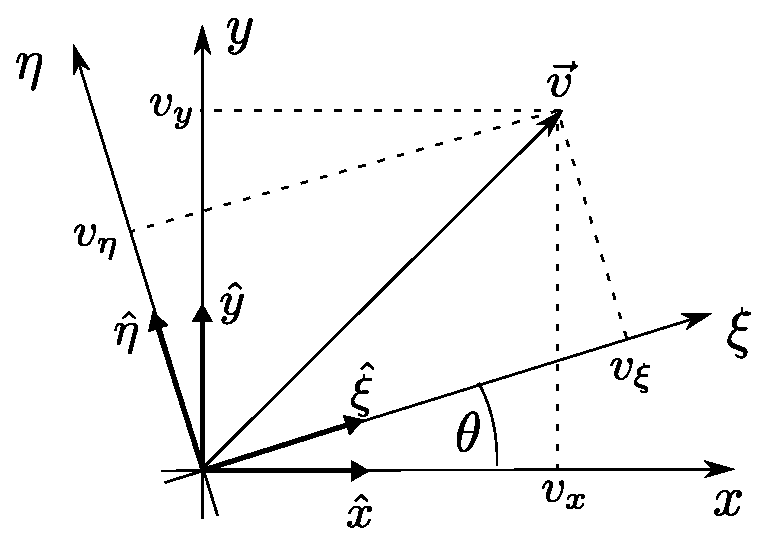
\includegraphics[width=0.95\textwidth]{./fig/rotation}
\end{center}
\end{minipage}
\end{tabular}
 
 
 
 
 
 
 
 
 
 
 



 \paragraph{Osservazione.}
 Gli elementi della base e le componenti di un vettore si trasformano seguendo le regole
 \begin{equation}
 \begin{cases}
  \tilde{\bm{e}}_i = \hat{T}^k_i \bm{e}_k  = \hat{T}_{ik} \bm{e}_k = T_{ki} \bm{e}_k\\
  \tilde{v}^i      = T^i_k v^k             = T_{ki} v^k            = \hat{T}_{ik} v^k
 \end{cases}
 \label{eqn:trGen}
 \end{equation}
 Come giustamente osservato da alcuni di voi, i vettori delle basi e le componenti dei vettori
 seguono la stessa trasformazione: questo è vero nel caso di rotazioni, poichè $\hat{T}:=T^{-1}=T^T$,
 in componenti $\hat{T}_{ik} = T_{ki}$ (osservate le relazioni qui sopra (\ref{eqn:trGen}) e come questo implica
 l'uguaglianza delle trasformazioni dei vettori della base e delle componenti). 
 Dalle relazioni trovate è immediato ricavare le trasformazioni inverse
 \begin{equation}
 \begin{cases}
  \bm{e}_i = T_{ik} \tilde{\bm{e}}_k = \hat{T}_{ki} \tilde{\bm{e}}_k\\
  v^i      = T_{ik} \tilde{v}^k      = \hat{T}_{ki} \tilde{v}^k
 \end{cases}
 \end{equation}
 
 \noindent
 Quando lo spazio è di dimensione 2, come nel nostro esercizio, si possono esplicitare le trasformazioni
 (\ref{eqn:trGen})
 
 \begin{equation}
 \begin{cases}
  \tilde{\bm{e}}_1 =  \hat{T}_{11} \bm{e}_1 + \hat{T}_{12} \bm{e}_2 \\
  \tilde{\bm{e}}_2 =  \hat{T}_{21} \bm{e}_1 + \hat{T}_{22} \bm{e}_2 \\
 \end{cases}
 \qquad
 \begin{cases}
  \tilde{v}_1 =  \hat{T}_{11} v_1 + \hat{T}_{12} v_2 \\
  \tilde{v}_2 =  \hat{T}_{21} v_1 + \hat{T}_{22} v_2 \\
 \end{cases}
 \label{eqn:trGen2}
 \end{equation}
 
 \vspace{0.05cm}
 \begin{center}
 \rule{0.75\textwidth}{.4pt}
 \end{center}
 \vspace{0.2cm}
 
 Si torna all'esercizio per ricavare la matrice di rotazione $T$, con le convezioni usate nell'osservazione, sostituendo
 al sistema indicato con la tilde il sistema $(\xi,\eta)$.
 Confrontando le trasformazioni (\ref{eqn:trEse}) dell'esercizio con quelle generali (\ref{eqn:trGen2}),
 la matrice di rotazione $\hat{T}$ che fa passare da $(x,y)$ a $(\xi,\eta)$ e la sua 
 inversa  $T$ (che coincide con la trasposta) sono
 \begin{equation}
 \hat{T} = \begin{bmatrix} 
  \cos{\theta} & \sin{\theta} \\
 -\sin{\theta} & \cos{\theta} \\
 \end{bmatrix}
 \qquad
 T = \begin{bmatrix} 
  \cos{\theta} & -\sin{\theta} \\
  \sin{\theta} &  \cos{\theta} \\
 \end{bmatrix}
 \end{equation}
 
 Consideriamo ora un tensore $\bm{A}$ del secondo ordine. Un esempio di tensore del secondo ordine è il tensore degli sforzi, 
 che ha anche la proprietà di essere simmetrico, $A_{ij} = A_{ji}$. Si può scrivere il tensore $\bm{A}$ in componenti rispetto alle due basi

 \begin{equation}
 \begin{aligned}
  \bm{A} & = A_{kl} \bm{e}_k \otimes \bm{e}_l = \\
   & = {A}_{kl} \hat{T}_{ik} \hat{T}_{jl} \tilde{\bm{e}}_i \otimes \tilde{\bm{e}}_j \\
   & = \tilde{A}_{ij} \tilde{\bm{e}}_i \otimes \tilde{\bm{e}}_j \\
 \end{aligned}
 \end{equation}
 
 Ragionando sugli indici, ricordando che indici ripetuti si sommano, è possibile rappresentare la trasformazione
 $\tilde{A}_{ij} = {A}_{kl} \hat{T}_{ik} \hat{T}_{jl}$
 delle componenti di un tensore del secondo ordine in forma matriciale
 \begin{equation}
 \begin{aligned}
   \tilde{A} & = \hat{T} A \hat{T}^T = T^T A T \\
   A & = \hat{T}^T \tilde{A} \hat{T} = T \tilde{A} T^T \\
 \label{eqn:trasfT2}
 \end{aligned}
 \end{equation}
 dove si sono definite le matrici $A$, $\tilde{A}$ contenti le componenti $A_{ij}$, $\tilde{A}_{ij}$ con il primo
  indice indicante la riga, il secondo la colonna.
  
 Il tensore $\bm{A}$ dell'esempio può essere scritto esplicitando tutti termini come
 \begin{equation}
 \begin{aligned}
  \bm{A} & = A_{xx} \bm{\hat{x}} \otimes \bm{\hat{x}} + A_{xy} \bm{\hat{x}} \otimes \bm{\hat{y}} 
           + A_{yx} \bm{\hat{y}} \otimes \bm{\hat{x}} + A_{yy} \bm{\hat{y}} \otimes \bm{\hat{y}} = \\
         & = A_{\xi\xi} \bm{\hat{\xi}} \otimes \bm{\hat{\xi}} + A_{\xi\eta} \bm{\hat{\xi}} \otimes \bm{\hat{\eta}} 
           + A_{\eta\xi} \bm{\hat{\eta}} \otimes \bm{\hat{\xi}} + A_{\eta\eta} \bm{\hat{\eta}} \otimes \bm{\hat{\eta}}
 \end{aligned}
 \end{equation}
 
 Le quattro componenti in ciascuna delle due basi possono essere organizzate in due matrici, legate tra di loro
 dalla relazione (\ref{eqn:trasfT2})
 \begin{equation}
   \begin{bmatrix}
    A_{\xi \xi} & A_{\xi \eta} \\
    A_{\eta\xi} & A_{\eta\eta} \\
   \end{bmatrix} = 
   \begin{bmatrix} 
    \cos{\theta} &-\sin{\theta} \\
    \sin{\theta} & \cos{\theta} \\
   \end{bmatrix}
   \begin{bmatrix}
    A_{xx} & A_{xy} \\
    A_{yx} & A_{yy} \\
   \end{bmatrix}
   \begin{bmatrix} 
    \cos{\theta} & \sin{\theta} \\
   -\sin{\theta} & \cos{\theta} \\
   \end{bmatrix}
 \end{equation}
 
 \paragraph{Tensore degli sforzi, sforzo piano e direzioni principali.}
Vediamo ora un esempio pratico, ingegneristico, di quanto fatto fino ad ora.
 Durante il corso di Scienze delle costruzioni avete incontrato il cerchio di Mohr, utilizzabile in uno stato di sforzo piano 
 ($\tau_{xz} = \sigma_{xz} = 0$, $\tau_{yz} = \sigma_{yz} = 0$, $\sigma_{zz} = 0$) per
\begin{itemize}
 \item trovare il vettore sforzo agente su una superficie di normale $\bm{\hat{n}}$, noto il tensore degli sforzi
 \item trovare gli sforzi principali e le direzioni principali (per le quali le componenti di taglio sono nulle)
\end{itemize}
 Cerchiamo ora di trovare le direzioni principali (basta trovare una direzione, l'altra è perpendicolare, poichè il tensore
 è simmetrico, $A_{xy} = A_{yx}$), usando la trasformazione appena trovata per un tensore simmetrico $\bm{A}$.
  \begin{equation}
  \begin{aligned}
   \begin{bmatrix}
    A_{\xi \xi} & A_{\xi \eta} \\
    A_{\eta\xi} & A_{\eta\eta} \\
   \end{bmatrix} & = 
   \begin{bmatrix} 
    \cos{\theta} & \sin{\theta} \\
   -\sin{\theta} & \cos{\theta} \\
   \end{bmatrix}
   \begin{bmatrix}
    A_{xx} & A_{xy} \\
    A_{xy} & A_{yy} \\
   \end{bmatrix}
   \begin{bmatrix} 
    \cos{\theta} &-\sin{\theta} \\
   \sin{\theta} & \cos{\theta} \\
   \end{bmatrix} = \\
   & = \begin{bmatrix}
    A_{xx} \cos^2 \theta + A_{yy} \sin^2 \theta + 2 A_{xy} \cos \theta \sin \theta & 
      (-A_{xx} + A_{yy}) \cos \theta \sin \theta + A_{xy} ( \cos^2 \theta - \sin^2 \theta) \\
  (-A_{xx} + A_{yy}) \cos \theta \sin \theta + A_{xy} ( \cos^2 \theta - \sin^2 \theta) &
      A_{xx} \sin^2 \theta + A_{yy} \cos^2 \theta - 2 A_{xy} \cos \theta \sin \theta 
   \end{bmatrix}
 \end{aligned}
 \end{equation}
 La proprietà di simmetria del tensore è indipendente dal sistema di coordinate nel quale vengono scritte le componenti
  ($A_{\xi \eta} = A_{\eta \xi}$).
  Per trovare l'angolo del quale sono ruotati gli assi principali rispetto agli assi $(x,y)$ imponiamo che si annulli la
  componente fuori dalla diagonale nel sistema ruotato
  \begin{equation}
   A_{\xi \eta} = 0
  \end{equation}
  \begin{equation}
   0 = A_{xy} \cos {2\theta} - \dfrac{\sin{2\theta}}{2} (A_{xx}-A_{yy}) \quad \Rightarrow \quad
   \tan {2 \theta} = \dfrac{2 A_{xy}}{A_{xx}-A_{yy}}
  \end{equation}
 %
 Il problema oggetto di questo esercizio è equivalente alla ricerca degli assi principali di sforzo per uno stato di sforzo piano.
  Il risultato ricavato tramite le trasformazioni delle componenti dei tensori coincide con quello  già ottenuto nei corsi precedenti tramite l'equilibrio di un elementino di materiale, riassumibile nel diagramma del cerchio di Mohr. Avere in mente entrambi gli approcci è utile per non perdere il significato fisico di quello che si sta facendo.
 \newline \noindent 
  Un altro impiego della trasformazione precedente, sempre ``da strutturista'', un po' più avanzato, è la determinazione 
  delle caratteristiche di elementi di materiale in composito, partendo dalle proprietà delle lamine che vengono 
  usate per costruirlo.
  Le lamine hanno caratteristiche espresse nel proprio sistema di riferimento, che in generale ha orientazione diversa
  da lamina a lamina, e diversa da un sistema di riferimento per l'elemento strutturale.
 \newline \noindent 
 Queste poche righe non hanno pretese di completezza, ma vogliono attirare l'interesse su quanto abbiamo visto nelle ultime 4 ore,
  anche da parte di quelli che diventeranno ``strutturisti'' ma non solo.
  

% 
% 
% %\section{Algebra}
% 
% %\section{Calcolo}
% 
% 
% %\index{Gradiente}




